\setcounter{chapter}{2}

\chapter{Gradient Descent}

\label{chap:gradient}

\section*{What is gradient descent?}


    \subsection{Why do we need gradient descent?}

        In the last chapter, we used an \textbf{analytical} approach to solve the OLS and RR problems.
        
        By "analytical", we mean we got an \textbf{explicit} answer: an equation we can use to directly compute the correct answer.
        
        The trouble is, we can't always do this:
        
        \begin{itemize}
            \item Sometimes the problem or the loss function can't be \textbf{rearranged} into a simple \textbf{equation}. 
            
            \item Or, we have \textbf{too much} data, and directly computing the answer would take way \textbf{too long}.\\
        \end{itemize}
        
        \begin{concept}
            Most \vocab{problems} we come across cannot be solved \vocab{analytically}.
        \end{concept}
        
        Well, if we can't \textbf{directly} find the \textbf{best} answer, what's the next best thing? Finding a \textbf{better} solution than your current one.
        
        So, our mission is to gradually try to find a better and better answer. This type of approach has a couple benefits:
        
        \begin{itemize}
            \item It's \textbf{quicker} to see if we're using a good model: if we're making very little progress, we can \textbf{quit} early and try something else.
            
            \item If we don't need \textbf{all} of our data to get the answer, we don't need to spend as much time. If our answer is \textbf{good} and not getting better, we can \textbf{stop}.
            
            \item It's easier to find a \textbf{better} answer than the \textbf{best} answer: our equations will be \textbf{simpler}. In some case, it might not have even been \textbf{possible} without this gradual approach!\\
        \end{itemize}
        
        \begin{concept}
            When we can't reasonably find a \purp{best} answer, it's often easier to find a \gren{better} answer and gradually \gren{improve}.
            
            \vocab{Gradient descent} follows this philosophy: we gradually \purp{update} our solution to make it better and better.
        \end{concept}
        
        
        
    \subsection{How do we improve?}
    
        So, now, the question is: how do we \textbf{improve} our hypothesis? We'll be modifying our hypothesis $\theta$ by some amount:
            \note{We'll do the same for $\theta_0$, but we'll do it separately. We'll come back to that.}
        
        \begin{equation}
            \theta_{new} = \theta_{old} + \Delta \theta
        \end{equation}
        
        \begin{notation}
            In equations, we'll often use $\theta_{old}$ and $\theta_{new}$ to represent \gren{before} and \purp{after} we take a step.
            
            We will use this notation \textbf{elsewhere} in the class.
        \end{notation}
        
        So, we are interesting in $\Delta \theta$: how do we plan to change $\theta$? What does $\Delta \theta$ look like?
        
        Well, we want to modify
        
        \begin{equation}
            \theta = 
            \begin{bmatrix}
                \theta_1 \\ \theta_2 \\ \vdots \\ \theta_d
            \end{bmatrix}
        \end{equation}
        
        So, we want to modify each of those terms.
        
        \begin{equation}
            \theta 
            = 
            \begin{bmatrix}
                \theta_1 \\ \theta_2 \\ \vdots \\ \theta_d
            \end{bmatrix}
            +
            \begin{bmatrix}
                \Delta \theta_1 \\ \Delta \theta_2 \\ \vdots \\ \Delta \theta_d
            \end{bmatrix}
        \end{equation}
        
        So, we have our total change!
        
        \begin{equation}
            \Delta \theta 
            = 
            \begin{bmatrix}
                \Delta \theta_1 \\ \Delta \theta_2 \\ \vdots \\ \Delta \theta_d
            \end{bmatrix}
        \end{equation}
        
        Notice that the shape of this change matches the shape of $\theta$: $(d \times 1)$.\\
        
        \begin{concept}
            We need a \purp{separate} term $\Delta \theta_i$ for each $\theta_i$ we want to \gren{improve}.
            
            So, a vector of the \purp{total} change, $\Delta \theta$, needs to have the \gren{same shape} as $\theta$: $(d \times 1)$.
        \end{concept}
        
        
    \subsection{The name: "gradient descent"}
    
        Our goal is to gradually \textbf{decrease} $J$, step-by-step. We do this using the \textbf{gradient}, hence "gradient descent". Why the gradient? We'll discuss that later.
        
        But why the word "\textbf{descent}"? 
        
        Our intuition is to imagine $J$ as having a \textbf{height} at every input value. If you combine all of these different points, you get a \textbf{surface}, like the surface of a hill.
        
        \begin{figure}[H]
            \centering
                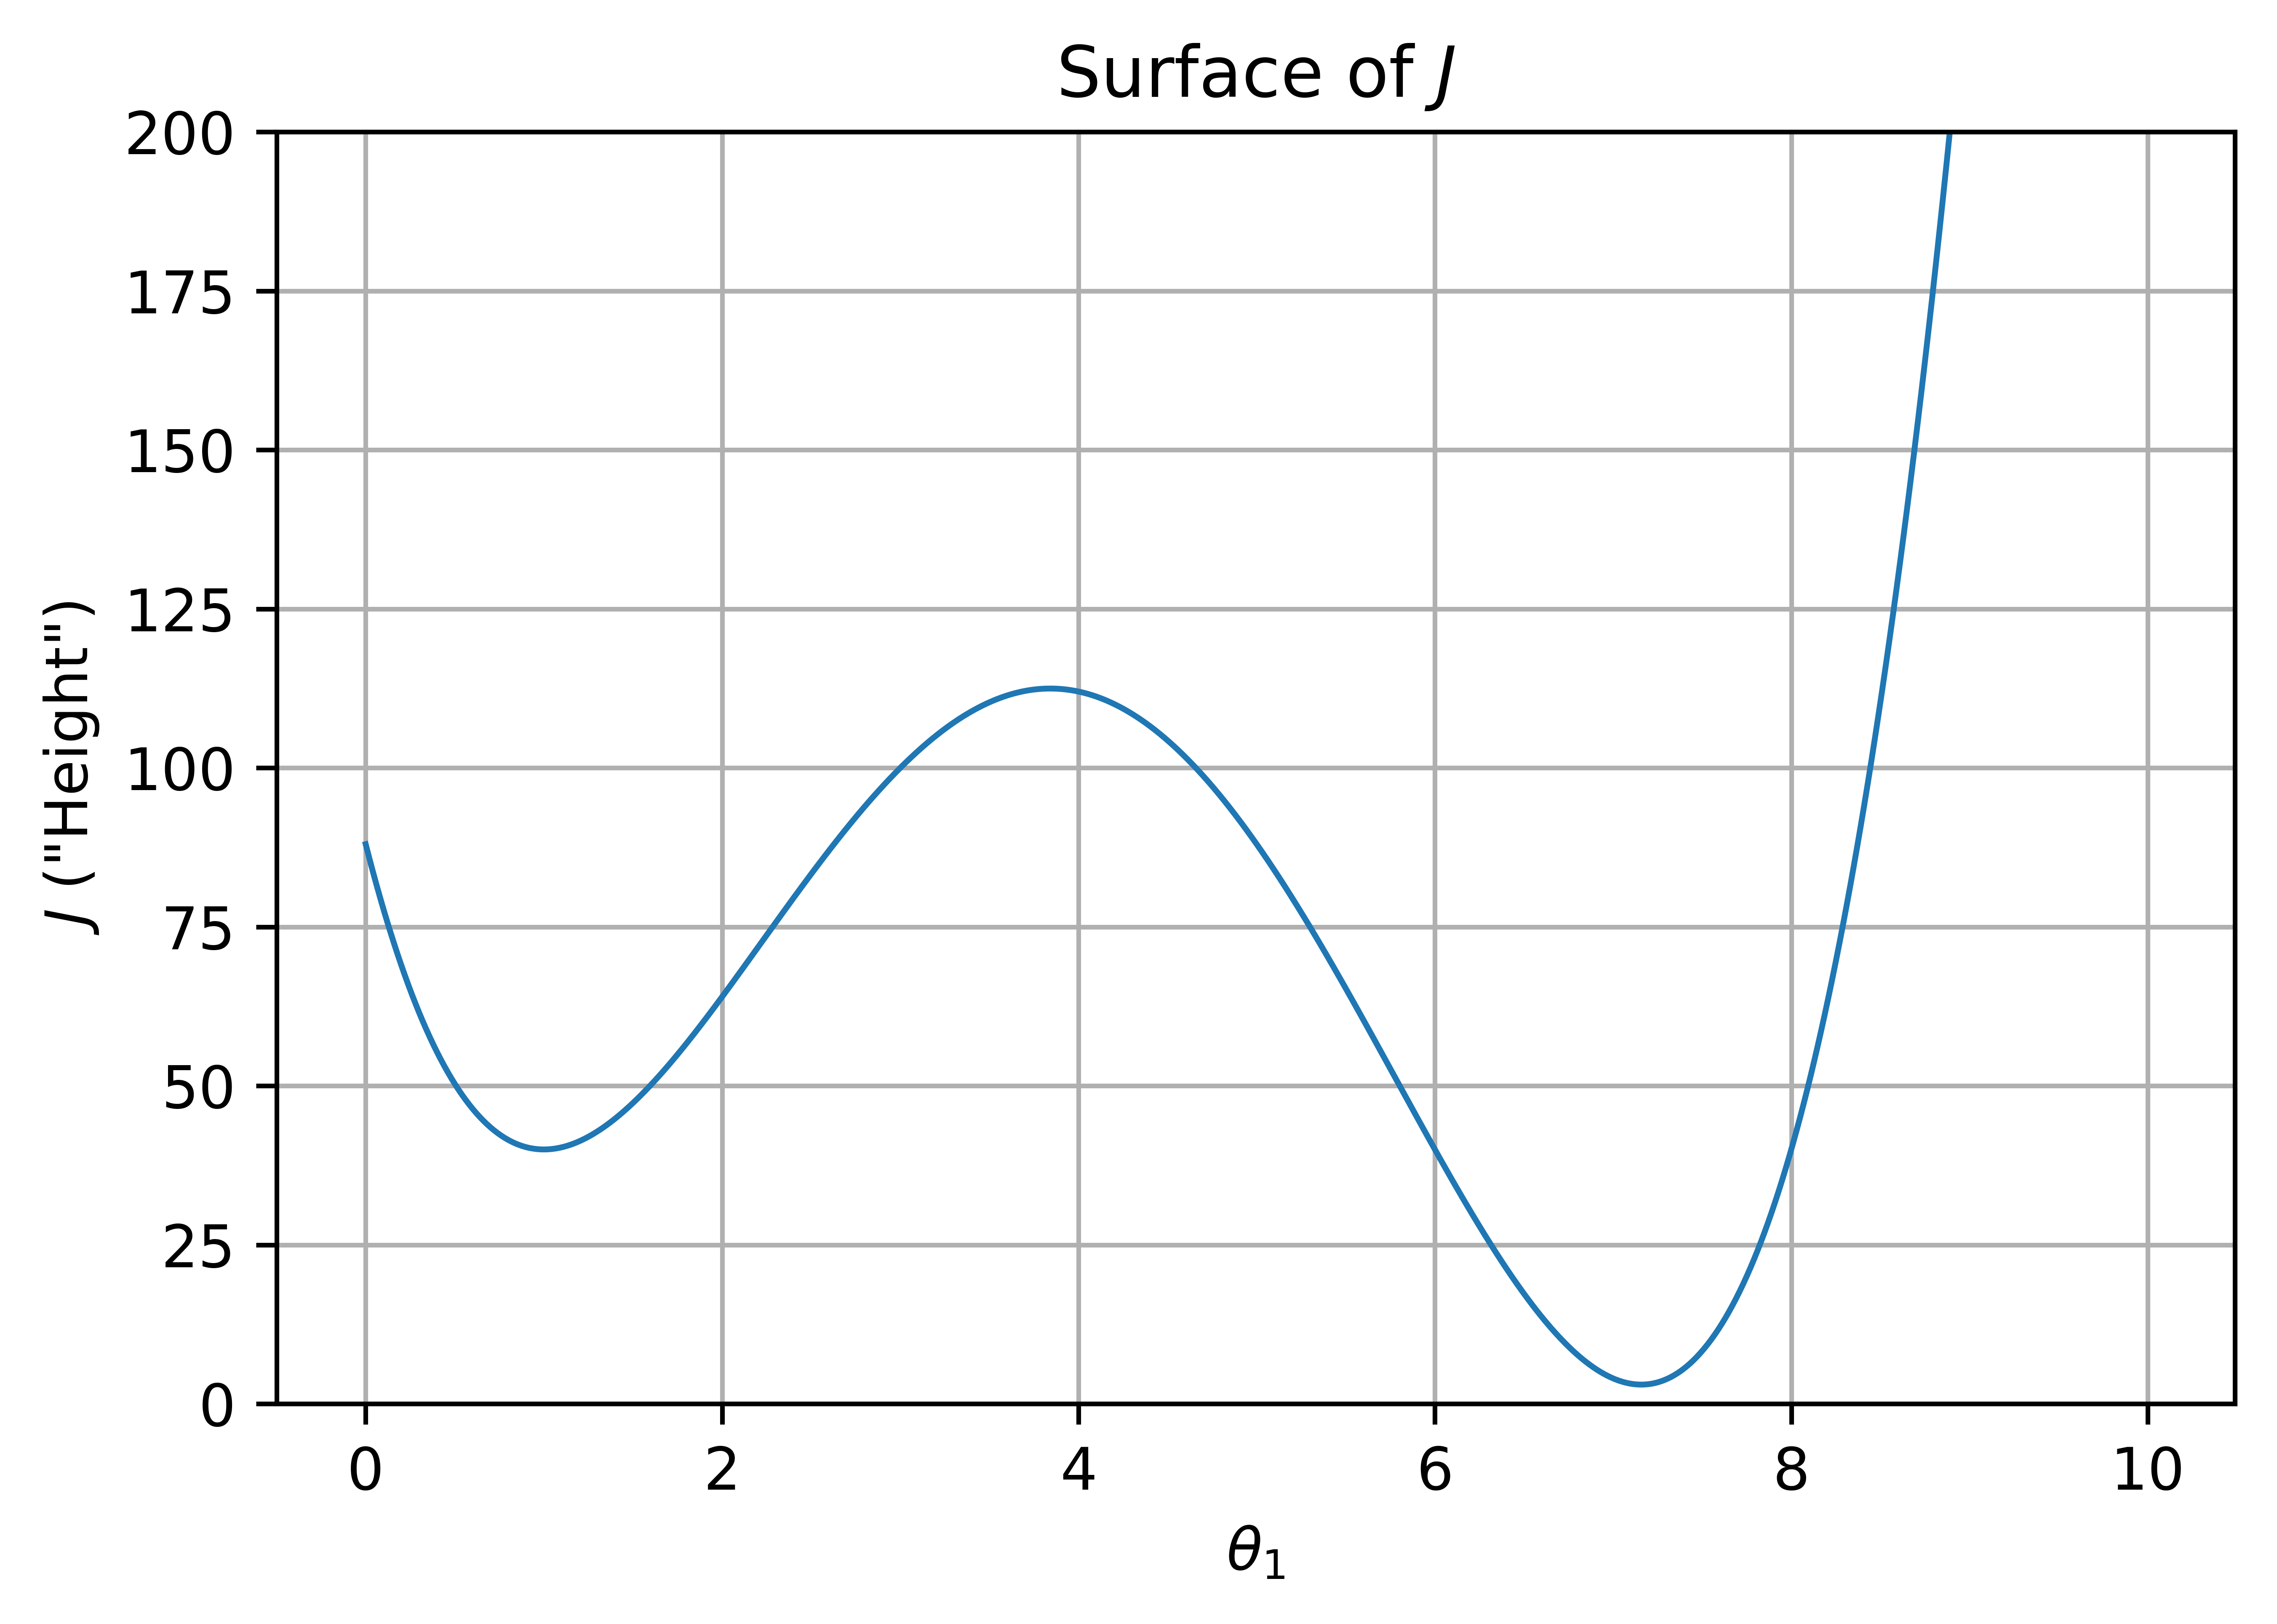
\includegraphics[width=70mm,scale=0.5]{images/gradient_descent_images/Surface_of_J.png}
            
            \caption*{You can imagine this like some hills we want to "descend".}
        \end{figure}
        
        Then, decreasing $J$ is moving \textbf{down} the the function, similar to rolling a ball down a hill. In other words, we \textbf{descend} the hill.
        
        \begin{figure}[H]
            \centering
                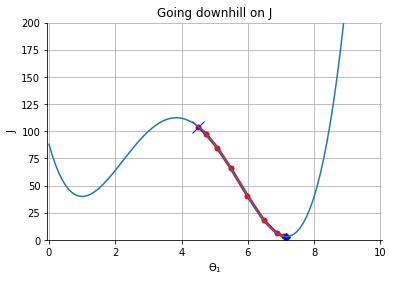
\includegraphics[width=70mm,scale=0.5]{images/gradient_descent_images/going_downhill.png}
            
            \caption*{Like this! Starting from the blue "X", moving 'downhill'.}
        \end{figure}
        
    \subsection{Input Space vs. Parameter Space}
    
        One more thing to note: we have two similar situations.
        
        \begin{itemize}
            \item $J$ is a \textbf{function} with $\theta$ as an \textbf{input}: $J(\theta)$.
            
            \item $h$ is a \textbf{function} with $x$ as an \textbf{input}: $h(x)$. 
        \end{itemize}
        
        In both cases, we can imagine the \textbf{output} as the "\textbf{height}" of our function: the \textbf{hill} we mentioned before. This \textbf{physical} intuition is useful to \textbf{gradient descent}.
        
        But, what about \textbf{input} to our function? That's the x-axis our hill is floating above:
        
        \begin{itemize}
            \item With $h(x)$, our x-axis was our \textbf{input space}, all possible $x_1$ values: the "space" containing all of our possible inputs.
            
            \item With $J(\theta)$, our x-axis is the \textbf{parameter space}, all possible $\theta$ values. We also called this our "\textbf{hypothesis space}".
                \note{We're assuming 1-D right now for simplicity. If we were 2-D, we'd have an entire 2D grid under our hill!}\\
        \end{itemize}
        
        \begin{definition}
            The \vocab{parameter space} is our set of all \gren{possible} parameter combinations.
            
            This is the same as the \vocab{hypothesis space}, because our parameters \gren{define} our hypothesis.
            
            When we \gren{optimize} our hypothesis, we are "\purp{exploring}" the hypothesis space. 
        \end{definition}
        
        This also gives us an idea of which hypotheses are "\textbf{similar}": those which are \textbf{closer} in parameter space (which we used, when we were doing regularization $\norm{\theta-\theta_{old}}$).
        
        This is the \textbf{space} we're exploring, as we try to move \textbf{downhill}. \\
        
        \begin{clarification}
            Pay attention to your \purp{axes}! 
            
            Sometimes, we're doing a 2-D or 3-D plot of $J$, and our inputs are $\theta_k$. Other times, we're plotting hypothesis $h$, with our axes $x_i$.
            
            These two plots could have the same surface, but they \gren{represent} completely different things.
        \end{clarification}
        

        
        

        
\pagebreak

%%%%%%%%%%%%%%%%%%%%%%%%%%%%%%%%%%%%%%%%%%%%%%%%%%%%%%%%%%%%%%%%%%%%%%%%%%%%%%%%%%%%%%%%%%%
\section{Gradient Descent in One Dimension}

    \subsection{Derivatives (Review)}
    
        Here, we'll use some concepts from \textbf{calculus}.
        
        We'll make improvements in small \textbf{steps}. And, we measure our improvement against the \textbf{loss function}, $J$: that's what we want to \textbf{optimize}.
        
        In calculus, we found that, over \textbf{small} enough steps, you can \textbf{approximate} as function as a straight line.\\
        
        \begin{figure}[H]
            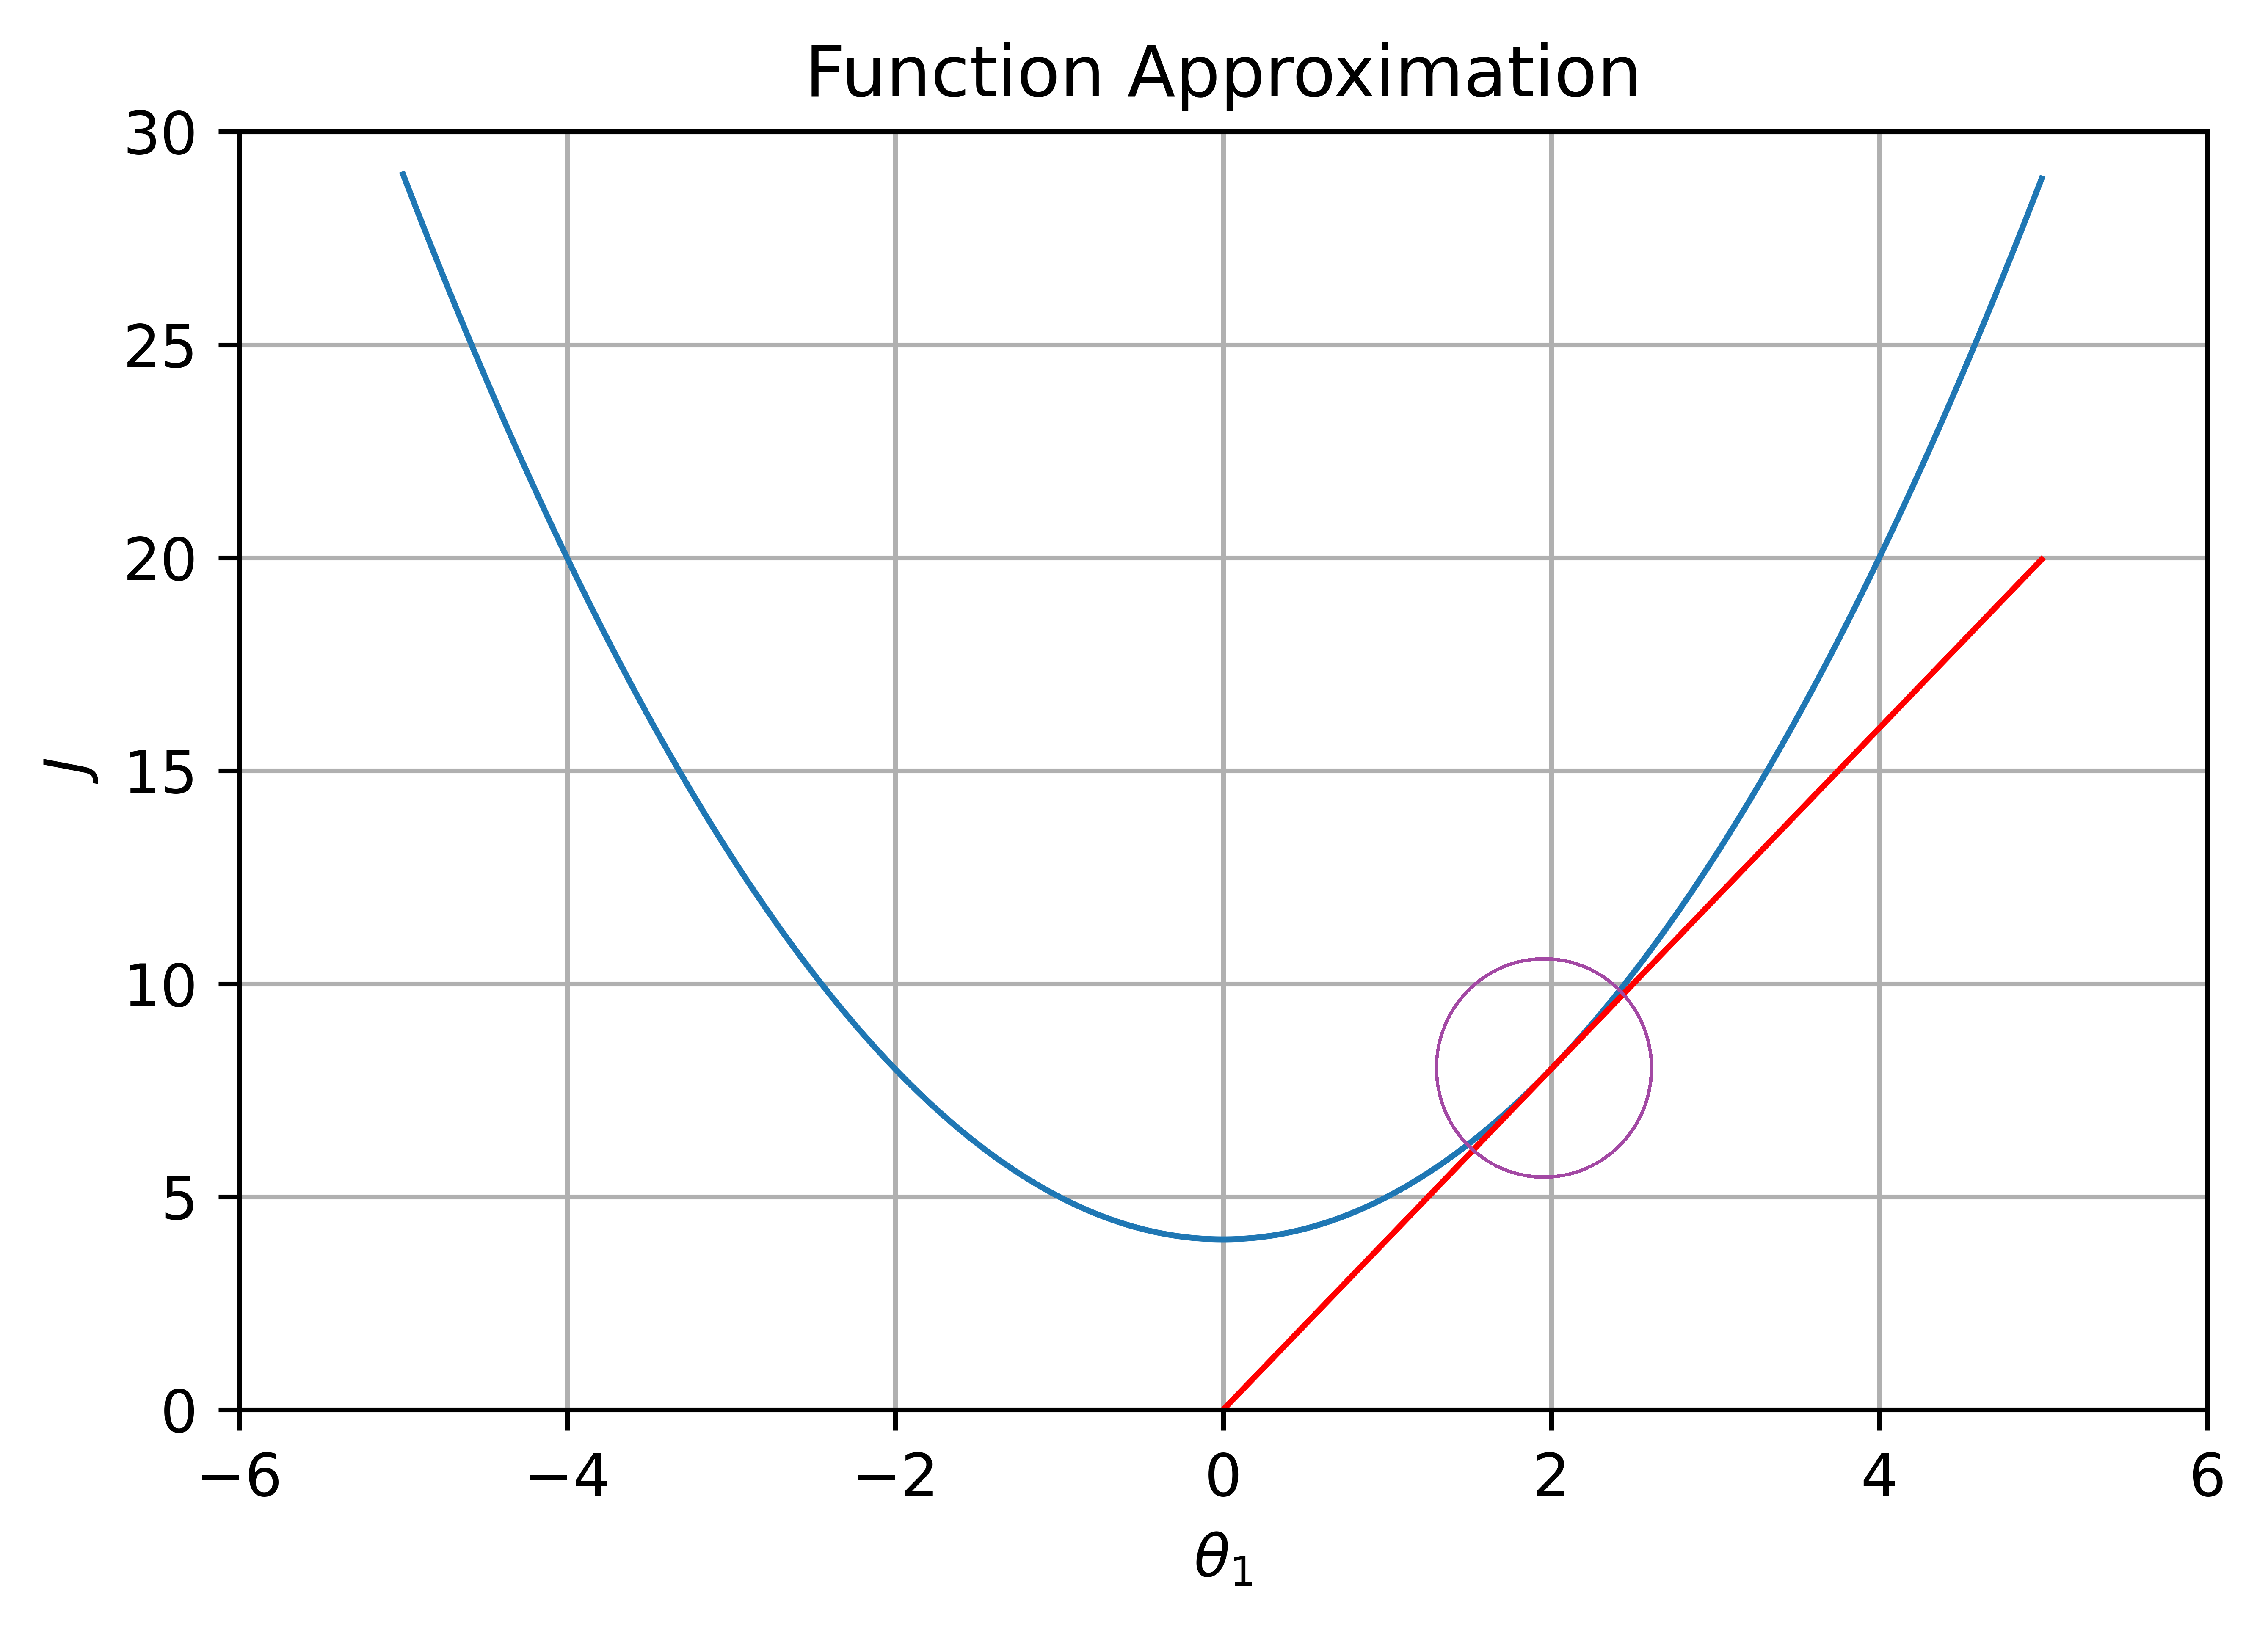
\includegraphics[width=70mm,scale=0.5]{images/gradient_descent_images/function_approximation_linear.png}
            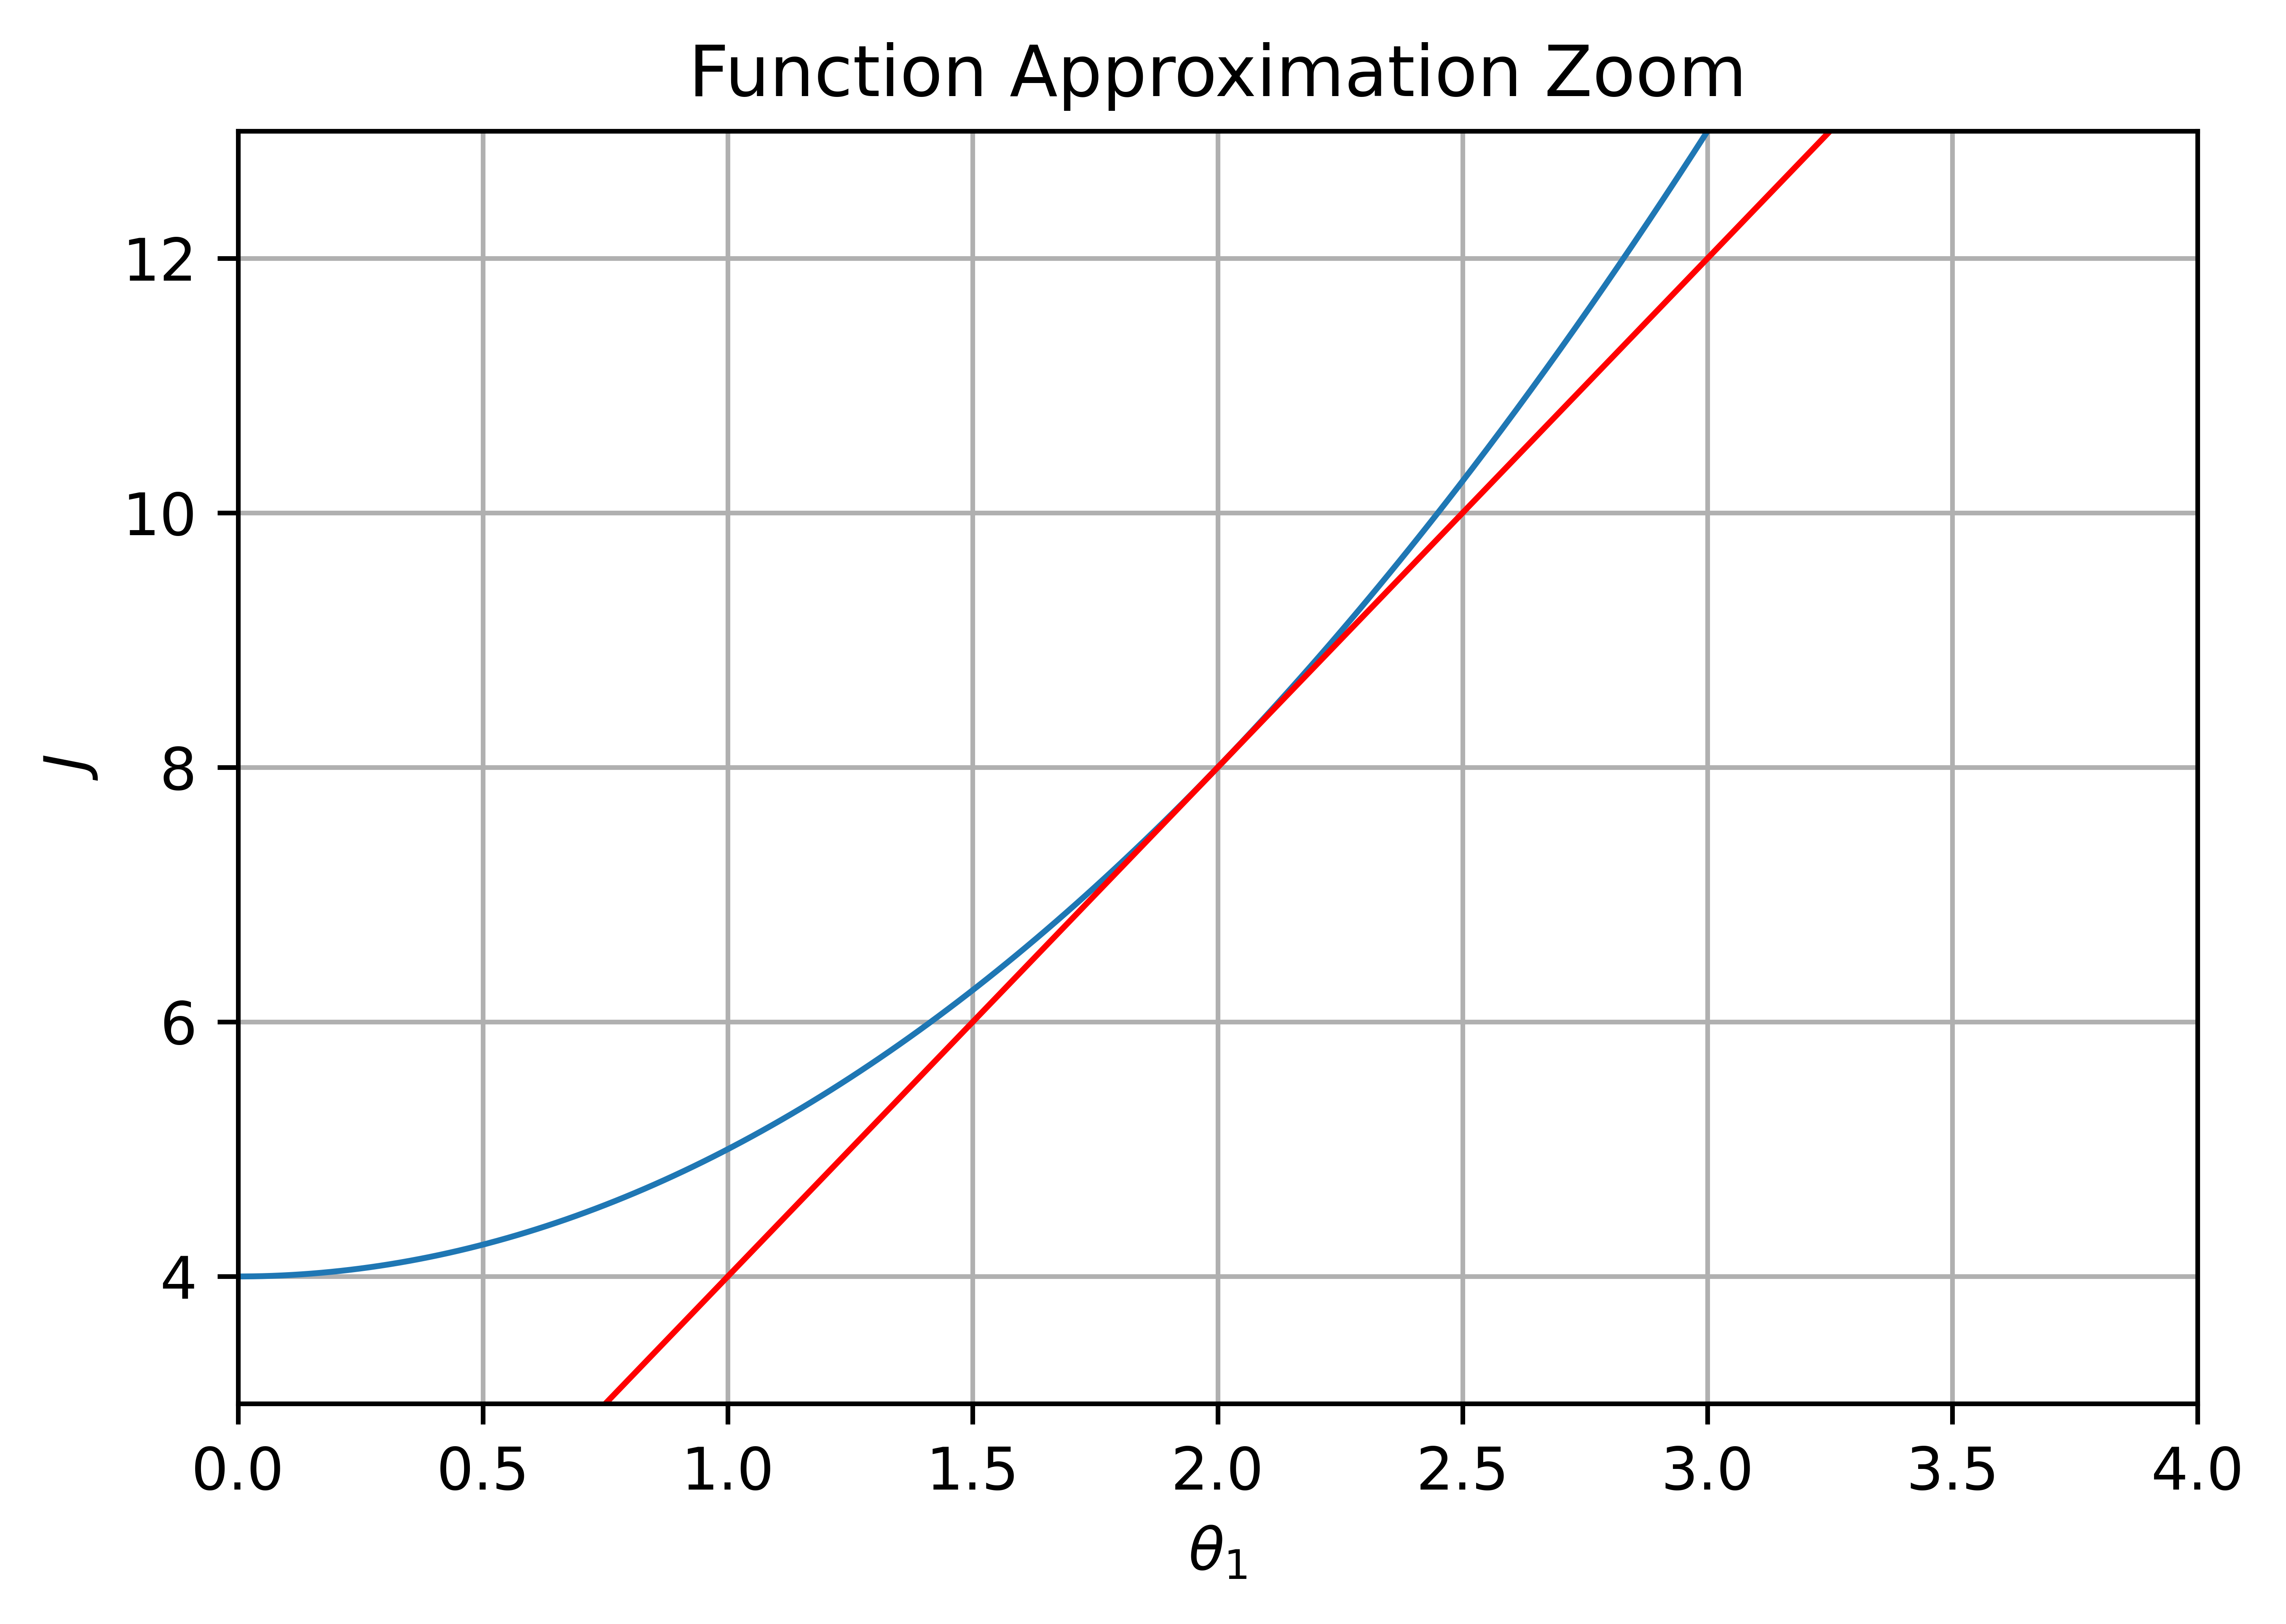
\includegraphics[width=70mm,scale=0.5]{images/gradient_descent_images/function_approximation_linear_zoom.png}
            
            \caption*{It looks more like a line as we zoom in: hence the \textbf{local} approximation.}
        \end{figure}
        
        %%Insert figure
        
        \begin{concept}
            A \gren{smooth} (enough) function can be \purp{approximated} with a \vocab{straight line} if you \purp{zoom} in on it enough.
            
            Looking at it this way is called a \vocab{local} view.
        \end{concept}
        
        
        
    \subsection{Optimize with Derivatives: 1-D}
        
        This gives us the \textbf{slope} of the function locally. Last chapter, we used $\deriv{J}{\theta}=0$ to get our \textbf{minimum}.
        
        But, let's not get too greedy - we want to \textbf{improve} our hypothesis, \textbf{not} immediately try to find the \textbf{best} one.
            \note{Because the best one might be expensive to find this way!}
        
        Well, what does our slope tell us? It tells us:
        
        \begin{itemize}
            \item How quickly $J$ changes
            \item Whether it \textbf{increases} or decreases as we change $\theta$
        \end{itemize}
        
        That second one tells us \textit{how to change} $\theta$: we want to move in the direction that \textbf{decreases} $J$.
        
        If the slope is \textbf{positive}, then we want to \textbf{decrease} $\Delta \theta$: the sign of $\Delta \theta$ is the opposite of our desired change!
        
        \begin{figure}[H]
            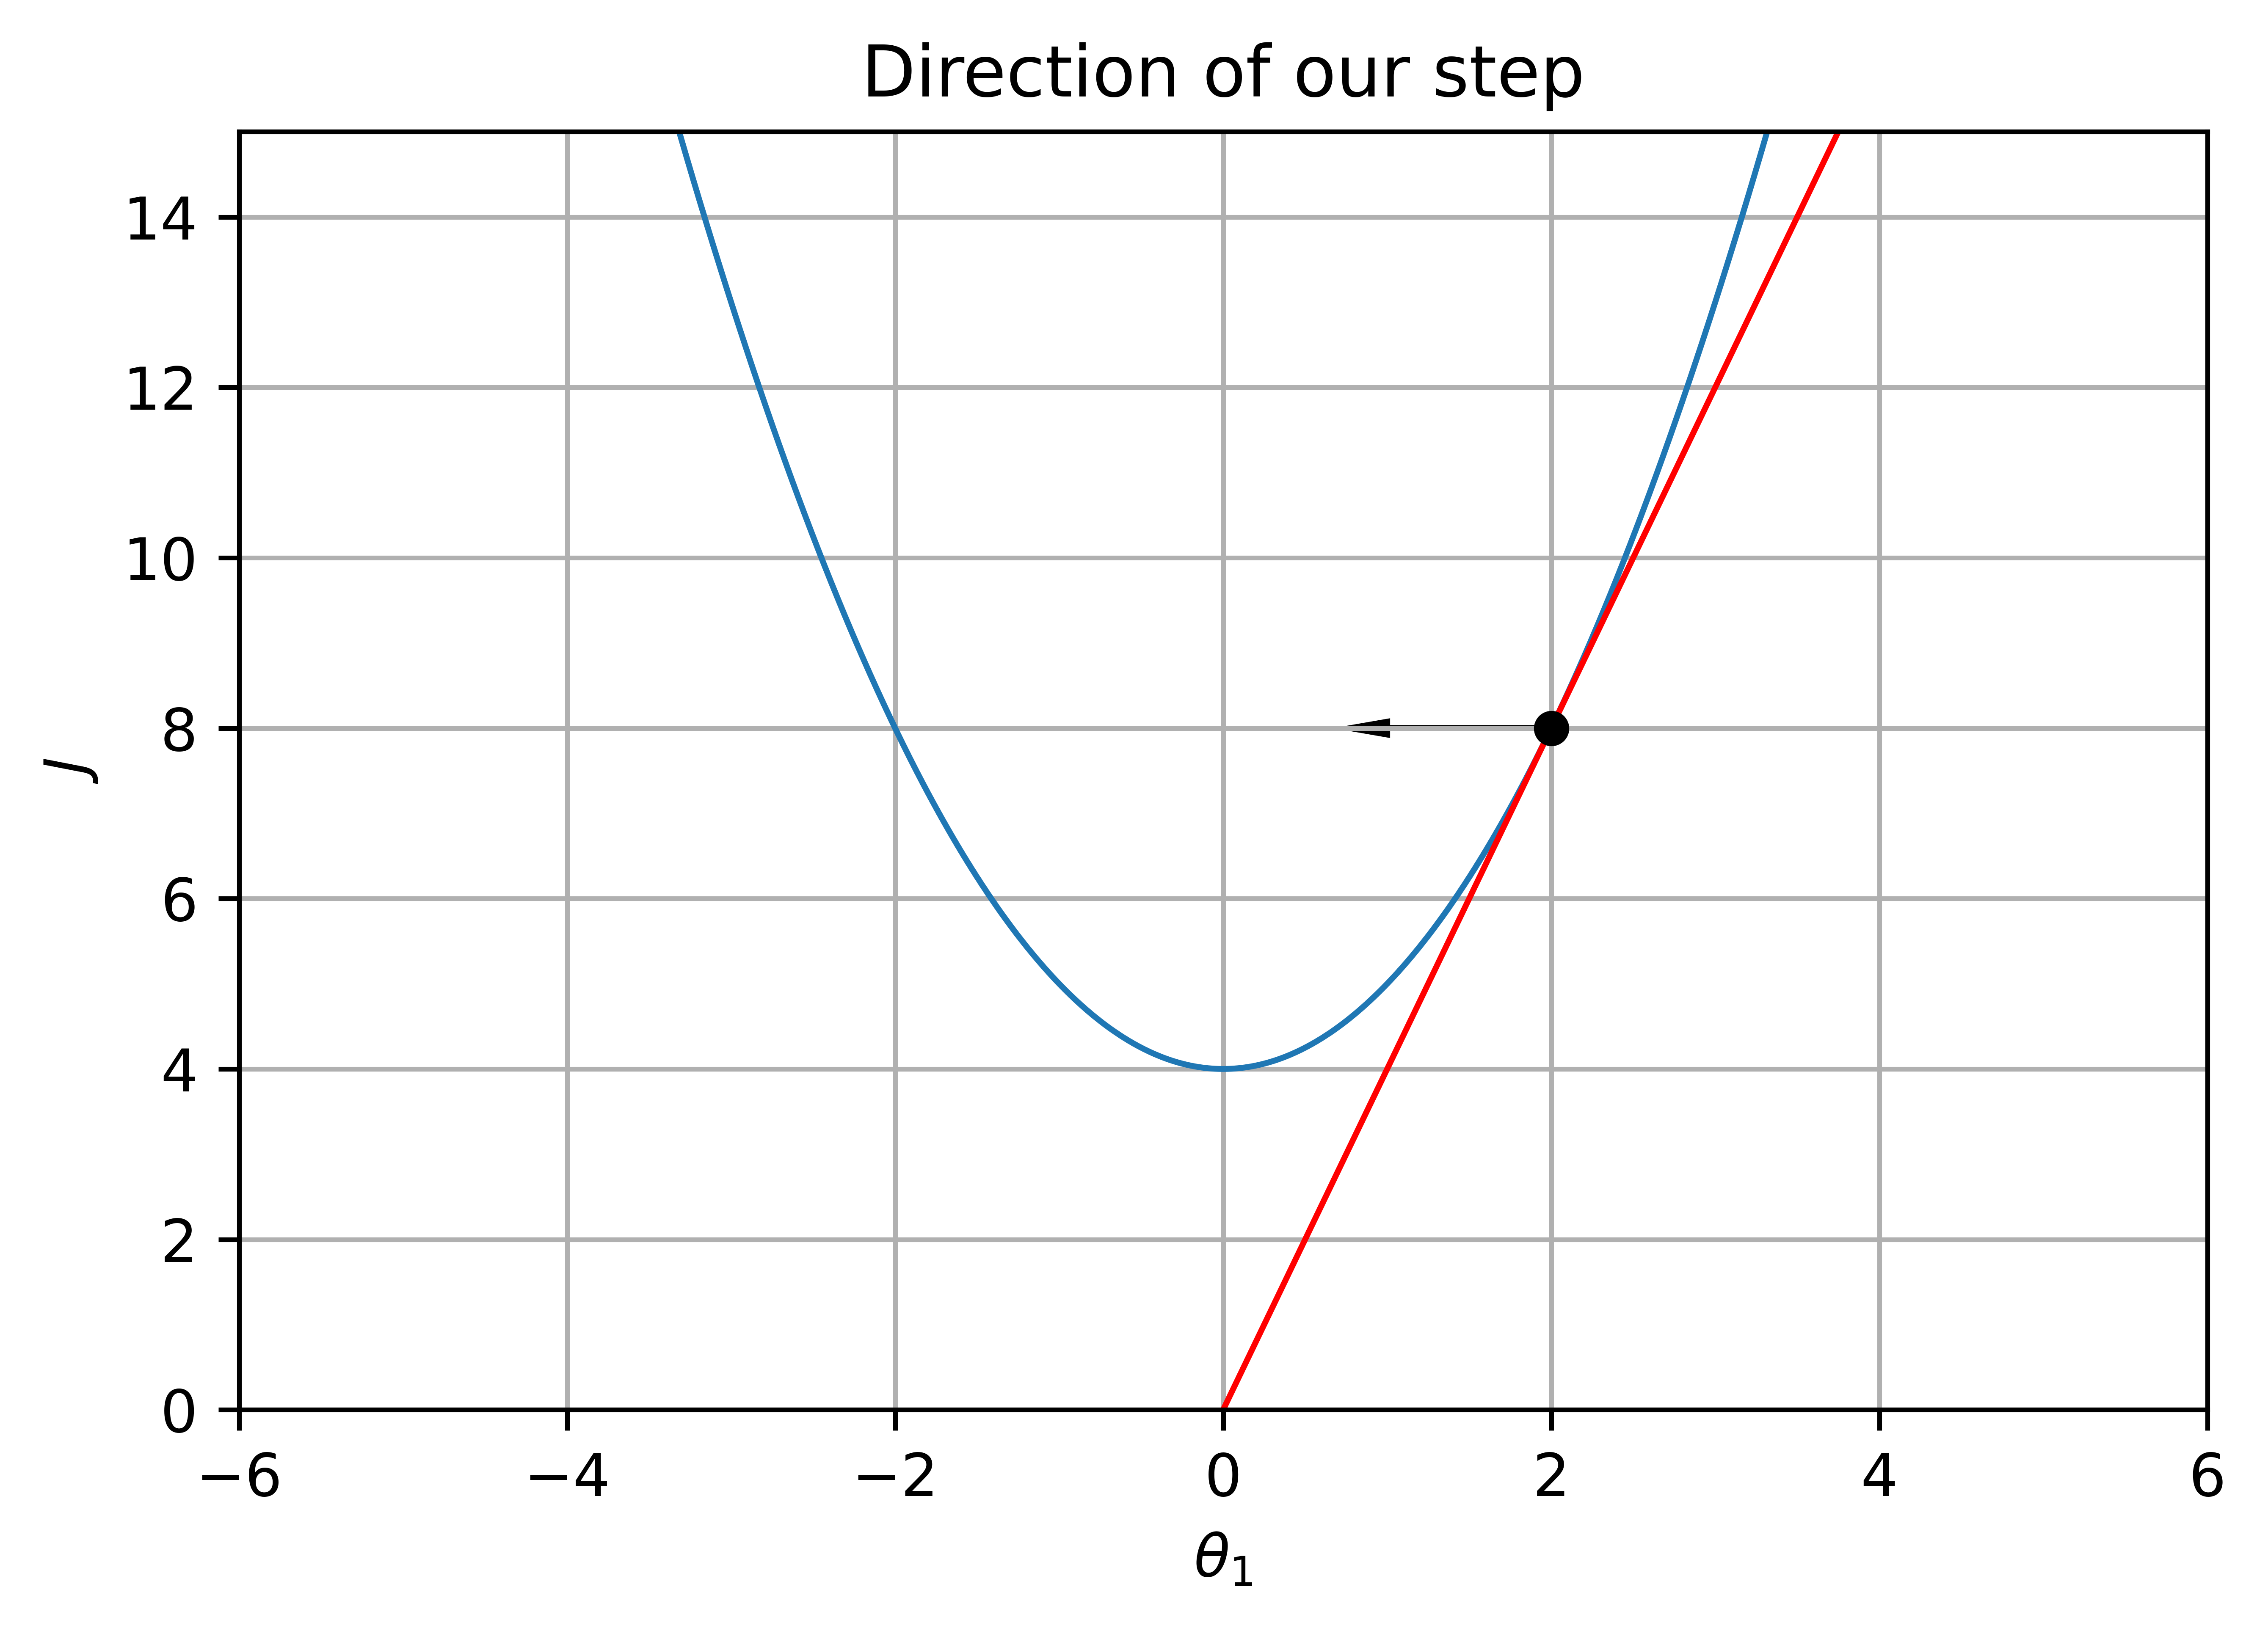
\includegraphics[width=70mm,scale=0.5]{images/gradient_descent_images/taking_a_step.png}
            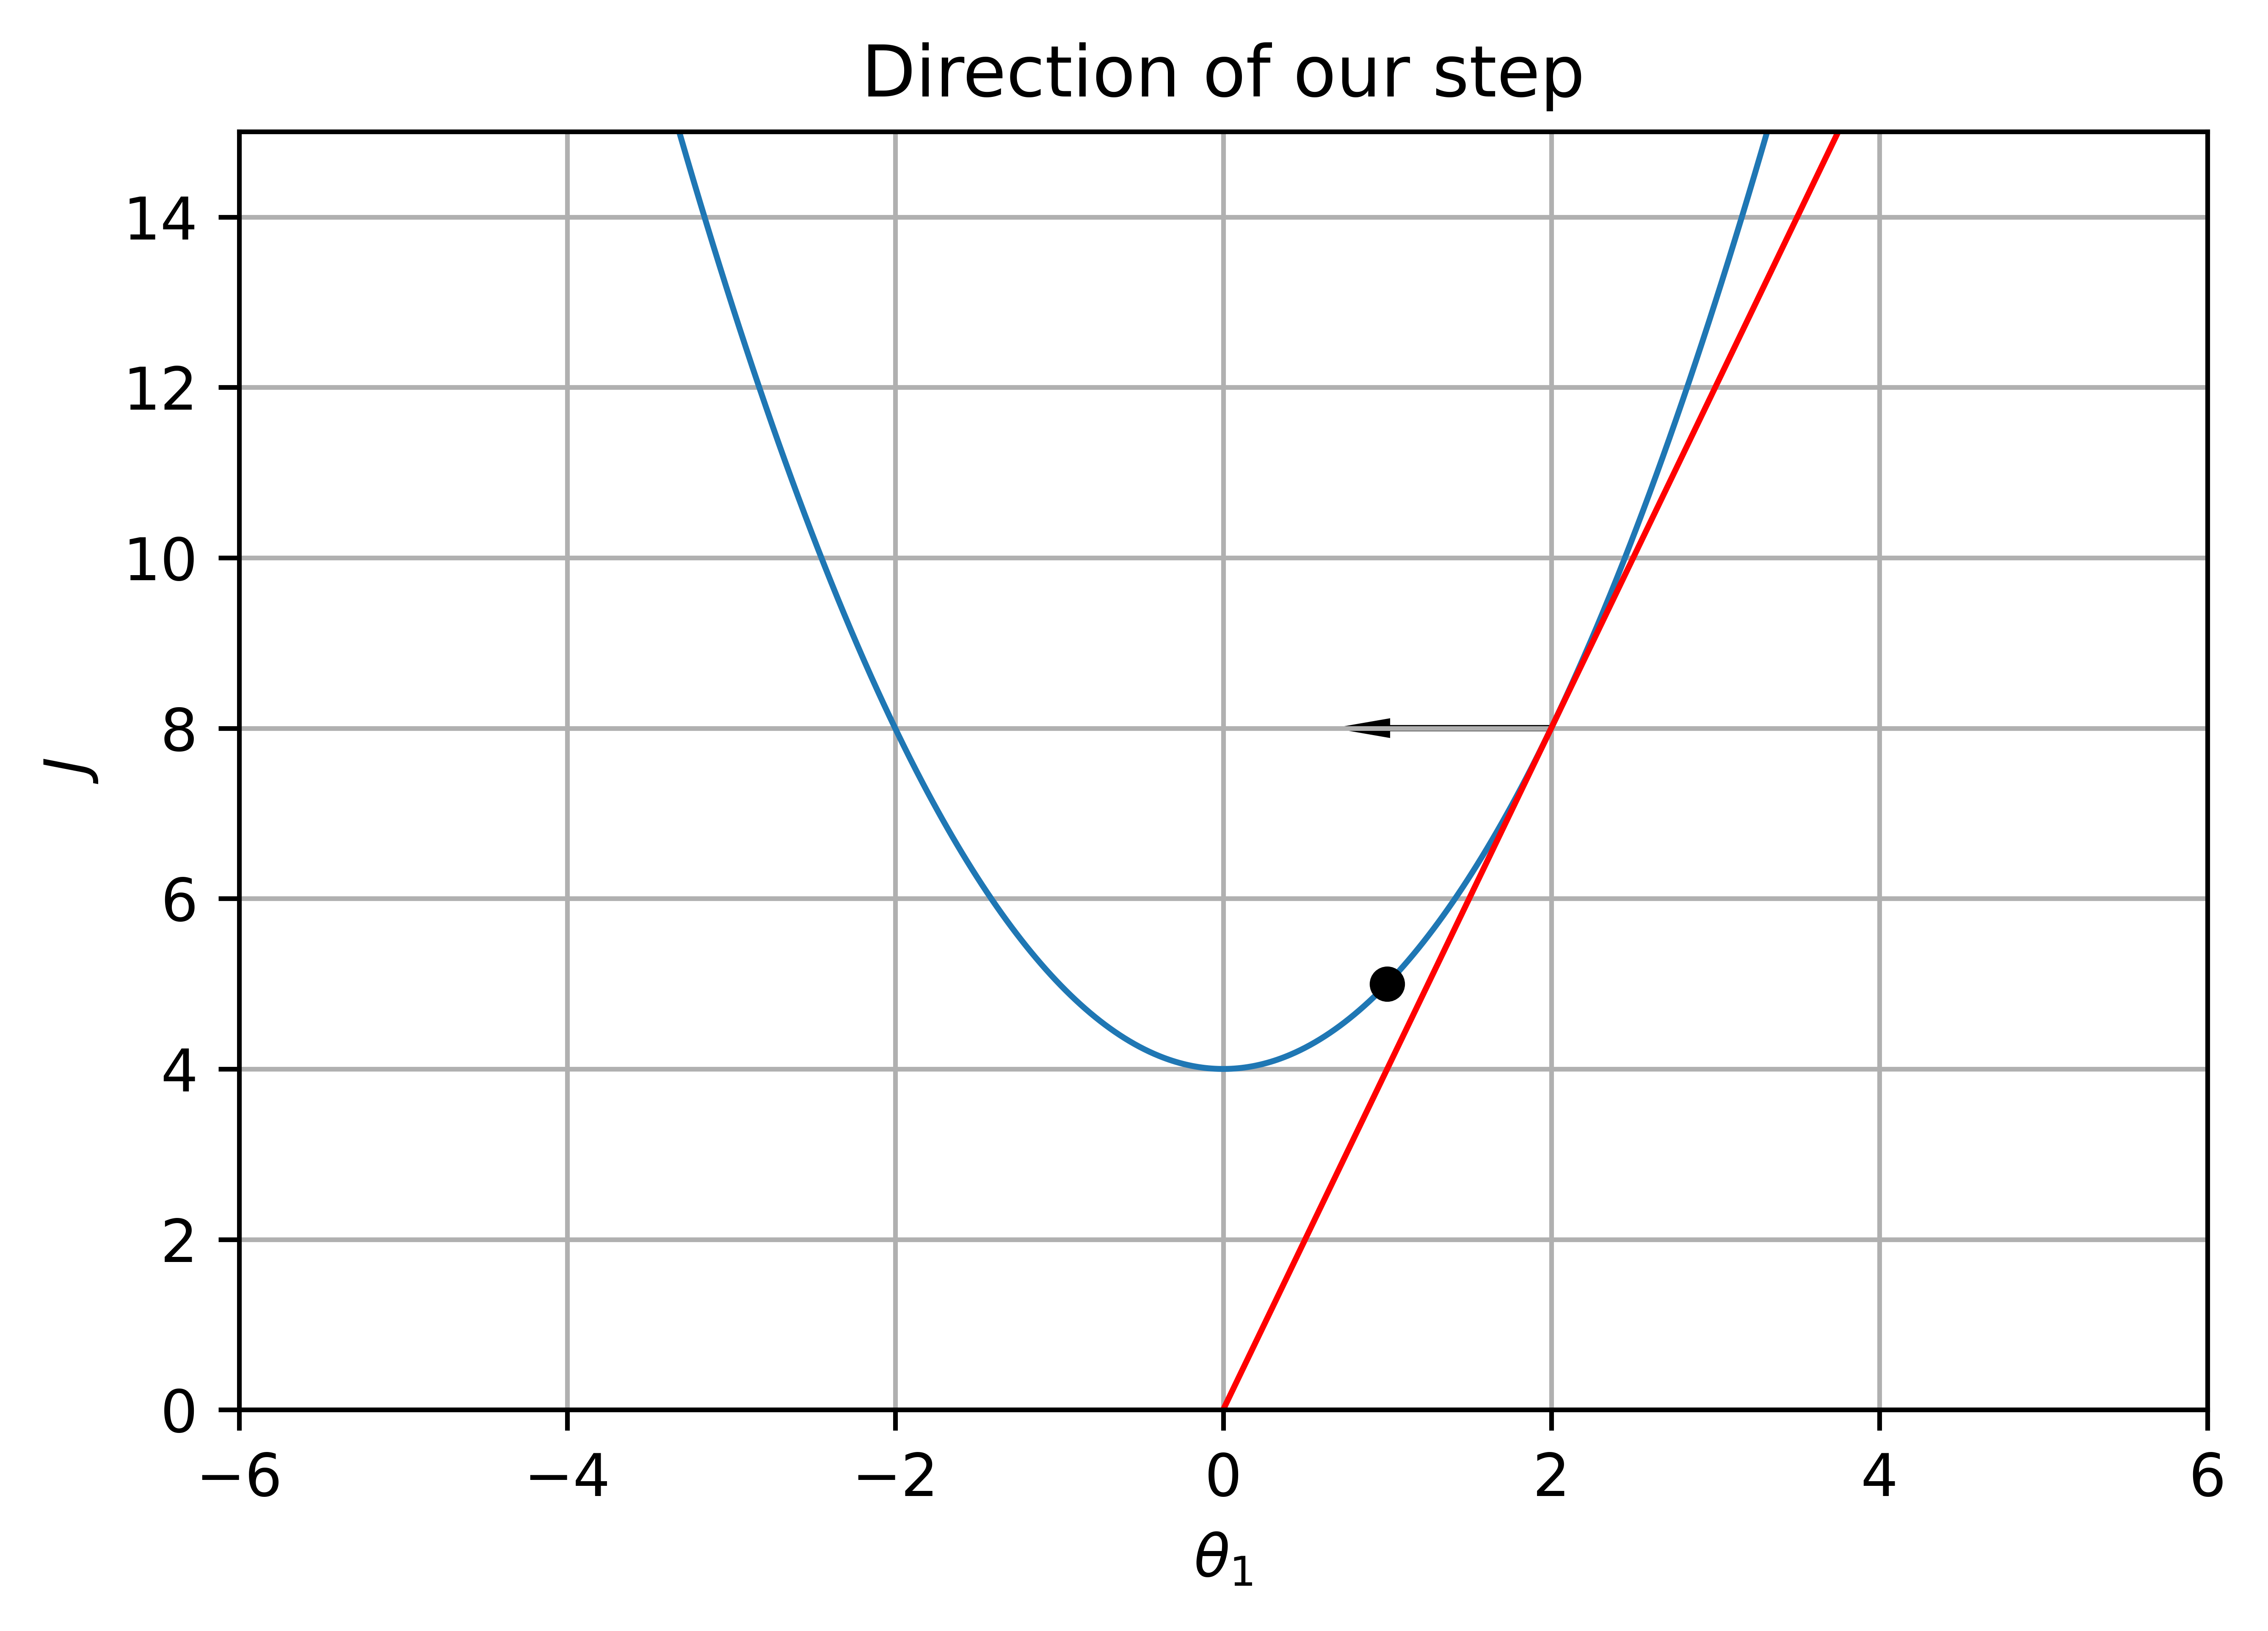
\includegraphics[width=70mm,scale=0.5]{images/gradient_descent_images/took_a_step.png}
            
            \caption*{Our slope is \textbf{positive}. We want to \textbf{decrease} our function, so we move in the \textbf{negative} direction, and "fall down" the surface.}
        \end{figure}
        
        And so, for now, we have
        
        \begin{equation}
            \Delta \theta = -\deriv{J}{\theta}
        \end{equation}\\
        
        \begin{concept}
            In \vocab{1-D}, you can use the \vocab{derivative} to \gren{optimize} our function $J$.
            
            The \purp{derivative} tells us how to immediately adjust $\theta_i$ to \gren{improve} our $J$ \purp{locally}: we move in the \gren{opposite direction}.
        \end{concept}
        
        This gives us a procedure for optimizing $J$: get the derivative $J'(\theta)$, and repeatedly adjust $\theta$ in the opposite direction until you're satisfied.
            \note{We'll need to pick a condition for being satisfied, but we'll get to this later}
        
        There's a certain way this feels like we're moving "\textbf{downhill}": we're moving "down" the slope, to try to find a local \textbf{minimum}.
        
    \subsection{Convergence}
    
        If you do this procedure with the above equation, though, you'll often run into \textbf{problems}. Why is that?
        
        Well, because each of your steps is too \textbf{big} or too \textbf{small}: we won't be able to find a \textbf{stable} answer, i.e. \textbf{converge}!
        
        What does it mean to \textbf{converge}? 
        
        It means we get a \textbf{single answer} after repeated steps: given enough time, we'll get \textbf{close as we want} to one number, and \textbf{stay there}.\\
        
        \begin{definition}
            If a sequence \vocab{converges}, then our result gets as \purp{close as we want} to a \gren{single number}, without going \purp{further away}.
        \end{definition}
        
        \miniex The numbers $1/n$: $\{ 1, \frac{1}{2}, \frac{1}{3}, \frac{1}{4}, \dots  \}$ converges to 0.
        
        If our answer \textbf{doesn't} converge, then it \textbf{diverges}. We can see why this might be bad: if we never \textbf{approach} a single answer, how do we know what value to \textbf{pick}?
        
    \subsection{Convergence: A little more formally (Optional)}
        
        Let's be more specific. Our sequence $S$ will converge to $r$.
        
        \begin{equation}
            S = \{ s_1, s_2, s_3, s_4, \dots \} 
        \end{equation}
        
        "As close as we want": let's say we want the maximum distance to be $\epsilon$. That means, no matter what $\epsilon>0$, we'll get closer at some point: $\abs{m-s_i}<\epsilon$
        
        \begin{equation}
            \abs{m-s_i}<\epsilon \text{ for some } i
        \end{equation}
        
        "And stay there": at some time $k$, we never move further away again:\\
        
        \begin{definition}
            If a sequence $S$ \vocab{converges} to $m$, then for all $\epsilon>0$, we can say
            
            \begin{equation}
                \abs{m-s_i}<\epsilon \text{ for all } i>k
            \end{equation}
        
        \end{definition}
        
        This is a "formal" definition of convergence.
        
    
    \subsection{Step size}
    
        If your steps are too \textbf{big}, your result might \textbf{diverge}: you make such big jumps, you move \textbf{away} from the minimum, and get worse.
            \note{Remember, if it \textbf{diverges}, it never \textbf{approaches} a single value!}
        
        \begin{figure}[H]
        \centering
            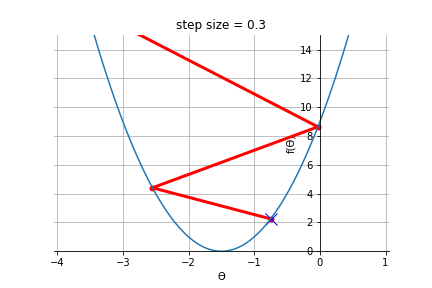
\includegraphics[width=70mm,scale=0.5]{images/gradient_descent_images/diverge.png}
        
        \caption*{We start at the blue "x" mark. Notice that, even though we try to move toward the minimum, we go too far and accidentally get further and further!}
        \end{figure}
        
        If they're too \textbf{small}, you might \textbf{converge} too slowly: it'll take way \textbf{too long} to make progress.
            \note{\textbf{Converging} means it successfully \textbf{approaches} an answer!}
        
        \begin{figure}[H]
        \centering
            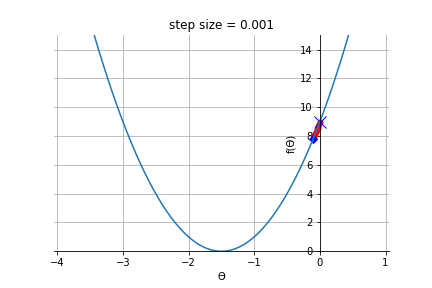
\includegraphics[width=70mm,scale=0.5]{images/gradient_descent_images/converge_slowly.png}
        
        \caption*{Our step size is too small: this is going to take too long!}
        \end{figure}
        
        In-between, it might converge, but \textbf{oscillate} a bunch: this can slow down getting an answer!
        
        \begin{figure}[H]
        \centering
            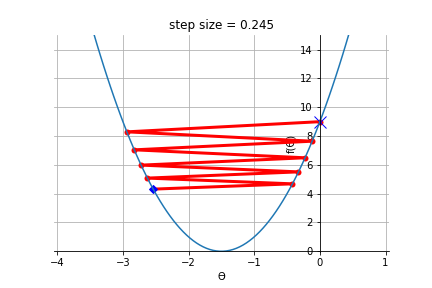
\includegraphics[width=70mm,scale=0.5]{images/gradient_descent_images/oscillate.png}
        
        \caption*{Most of our step is spent undoing the last step... we get better very slowly.}
        \end{figure}
        
        But, if we get the right step size, it'll converge nice and reasonably!
        
        \begin{figure}[H]
            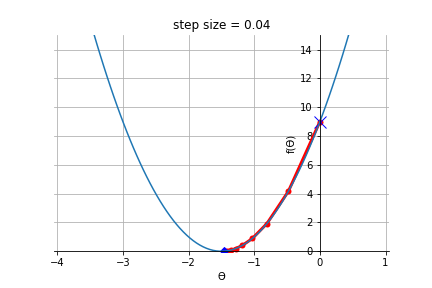
\includegraphics[width=70mm,scale=0.5]{images/gradient_descent_images/good_converge.png}
            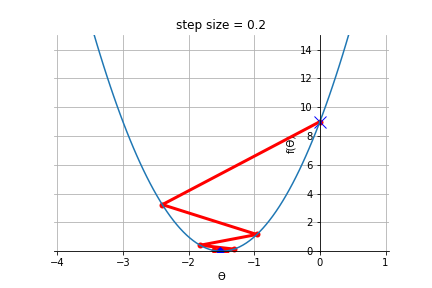
\includegraphics[width=70mm,scale=0.5]{images/gradient_descent_images/good_converge_oscillate.png}

            \caption*{Both of these look pretty good! One of them oscillating a bit is fine.}
        \end{figure}
        
        One question you might ask is, "\textbf{how much} oscillation is too much? Am I converging \textbf{fast enough}?" 
        
        This is a good question, but the simple answer is that there is \textbf{no objective answer}: it depends on what you \textbf{need} and how much \textbf{time} you have. But you should strive to do \textbf{better} when you can!\\
        
        \begin{concept}
            Using the \purp{wrong} step size can cause:
            
            \begin{itemize}
                \item Slow convergence
                \item Strong Oscillation
                \item Divergence
            \end{itemize}
            
            Which is why we \gren{adjust} the step size using $\eta$.
        \end{concept}
        
    \subsection{Step size $\eta$}
    
        Right now, our step size is at the mercy of $J'(\theta)$. But, we don't have to be: we could \textbf{scale} our step size up or down.
        
        We do this with our \textbf{scaling} factor (also called a \textbf{learning rate}), $\eta$.
        
        So, we can rewrite our \textbf{change} in $\theta$ as:
        
        \begin{equation}
            \Delta \theta
            = -\red{\eta}   \deriv{J}{\theta}
            = -\red{\eta}   J'(\theta)
        \end{equation}
        
        \begin{definition}
            Our step size parameter $\eta$, or \vocab{eta}, \purp{scales} how large each of our optimization steps are.
            
            If $\eta$ is bigger, we might \gren{learn} faster, but we also risk \purp{diverging}.
            
            Different values of $\eta$ are good for \gren{different situations}.
        \end{definition}
        
    \subsection{Our procedure}
    
        So, we have our parameter \textbf{update}, $\Delta \theta$. We'll start at $t=0$.
        
        Before, we represented the $\nth{i}$ \textbf{data point} with $\ex{x}{i}$. We'll reuse this \textbf{notation}.\\
        
        \begin{notation}
            Here, we're changing $\theta$ over \purp{time}: each step happens at $t=\{1,2,3, \dots \}$ so we need \gren{notation} for that. 
            
            We'll \gren{reuse} the notation from $\ex{x}{i}$, for the $\nth{i}$ data point.
            
            In this case, we'll do $\ex{\theta}{t}$: the value of $\theta$ after $t$ \purp{steps} are taken.
            
            Earlier, we \textbf{introduced} \blu{$\theta_{old}$} and \red{$\theta_{new}$}: these are \blu{$\ex{\theta}{t-1}$} and \red{$\ex{\theta}{t}$}.
        \end{notation}
        
        \miniex After \textbf{10 steps} of 1-D gradient descent, we have gone from $\ex{\theta}{0}$ to $\ex{\theta}{10}$.
        
        So, we move the \textbf{first} time using $J'(\ex{\theta}{0})$.
        
        Once we've moved in parameter space \textbf{one} time, though, our \textbf{derivative} has changed: we're in a different part of the \textbf{surface}.
        
        So, we'll take a \textbf{second} step with a \textbf{new} derivative, $J'(\ex{\theta}{1})$.
        
        We want to do this \textbf{repeatedly}. We'll take our equation
        
        \begin{equation}
            \theta_{new} = \theta_{old} + \Delta \theta
        \end{equation}
        
        And combine it with our \textbf{chosen} step size.\\
        
        \begin{kequation}
            In \vocab{1-D}, \vocab{Gradient Descent} is implemented as follows:
        
            At each time step $t$, we \purp{improve} our hypothesis $\theta$ using the following rule:
            
            \begin{equation*}
                \red{ \theta_{new} } = 
                \blu{ \theta_{old} } - \grn{\eta} J'( \blu{ \theta_{old} })
            \end{equation*}
            
            Using $\ex{\theta}{t}$ notation:
            
            \begin{equation*}
                \red{ \ex{\theta}{t} } = 
                \blu{ \ex{\theta}{t-1} } -
                \grn{\eta} J'( \blu{ \ex{\theta}{t-1} })
            \end{equation*}
            
            We repeat until we reach whatever our chosen \purp{termination condition} is.
        \end{kequation}
        
        We can also write it as:
        
        \begin{equation*}
                \red{ \theta_{new} } = 
                \blu{ \theta_{old} } - 
                \grn{\eta} 
                \left( \deriv{J}{ \blu{ \theta_{old} }} \right)
            \end{equation*}
        
        We've got our gradient descent \textbf{update} rule in 1-D!
    
    \subsection{Termination Conditions}
    
        When do we \textbf{stop}? We can't let it run forever.
        
        We have some options:
        
        \begin{itemize}
            \item Stop after a \textbf{fixed} $T$ steps.
                \begin{itemize}
                    \item This has the advantage of being \textbf{simple}, but how do you know what the \textbf{correct} number of steps is?
                \end{itemize}
            
            \item Stop when $\theta$ \textbf{isn't changing} much: $\big| \Delta \theta \big| < \epsilon$, for example.
            \begin{itemize}
                \item If our $\theta$ isn't changing much, our algorithm isn't \textbf{improving} our hypothesis much. So, it makes sense to stop: we've stabilized.
            \end{itemize}
            
            \item Stop when the \textbf{derivative is small}: $\big| J'(\theta) \big| < \epsilon$.
            \begin{itemize}
                \item Mathematically \textbf{equivalent} to our last choice. But a different \textbf{perspective}: if the slope is small, our surface is relatively \textbf{flat}, and we're near a \textbf{minimum} (probably).
                
                \item "The derivative is \textbf{small}" is weaker, but in the same spirit as "the derivative is \textbf{zero}", $J'(\theta)=0$, from last chapter.
            \end{itemize}
            
        \end{itemize}
        
    \subsection{Convergence Theorem}
    
        It turns out, if our function is \textbf{nice} enough, and we pick the \textbf{right} value of $\eta$, we can guarantee convergence!\\
        
        \begin{theorem}
            We want to optimize function $J$. If J is 
            \begin{itemize}
                \item Smooth enough
                \item Convex
            \end{itemize}
            
            And
            
            \begin{itemize}
                \item $\eta$ is small enough
            \end{itemize}
            
            Then gradient descent \textbf{will} converge to the \textbf{global minimum}!
        \end{theorem}
        
        "Small enough" seems vague, but it basically means, "an $\eta$ small enough to converge \textbf{exists}". 
            \note{If we want to say it in a mathy way, we can say "\textbf{there exists} an $\eta$ small enough to converge"} 
        
        Or, if your $\eta$ is too \textbf{big}, you can keep trying \textbf{smaller} ones, until it works. 
        
        This is amazing! We can \textbf{guarantee} a best solution in some cases!
        
    \subsection{Concavity}
    
        One requirement we haven't focused on "$J$ is \textbf{convex}". Why do we need $J$ to be convex?
        
        Well, if it's \textbf{concave}, there is no \textbf{global minimum}: it goes down forever!\\
        
        \begin{figure}[H]
        \centering
            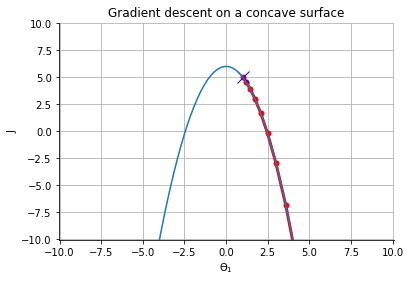
\includegraphics[width=70mm,scale=0.5]{images/gradient_descent_images/gradient_descent_on_a_concave_surface.png}
        
        \caption*{Our gradient just leads us downhill forever.}
        \end{figure}
        
        \begin{concept}
            If our function $J$ is \purp{concave}, then our result will not \purp{converge}: it will continue to \gren{decrease} more and more indefinitely.
        \end{concept}
        
        So, for future problems, let's assume it \textbf{doesn't} go down forever: if it was, then there is no best solution! We don't have a \textbf{valid} problem.
        
    \subsection{Local minima}
        
        Even if we don't have that problem, we have a \textbf{different} one:
        
        Gradient descent \textbf{gradually} improves our solution until it reaches one it's \textbf{satisfied} with. But, what if there are \textbf{multiple} solutions we could reach?
        
        Are they all equally good?
        
        \begin{figure}[H]
        \centering
            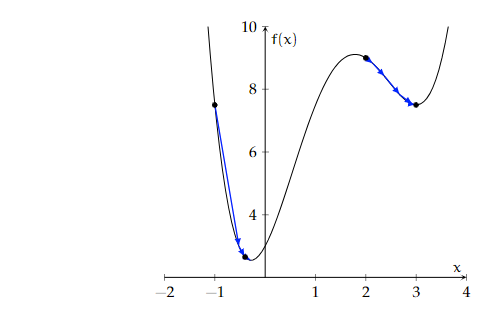
\includegraphics[width=70mm,scale=0.5]{images/gradient_descent_images/Two_Local_Minima.png}
        
        \caption*{Depending on your starting position (\textbf{initialization}), you could find a different local minimum!}
        \end{figure}
        
        Maybe not! So, if our function isn't \textbf{always convex}, we can end up with \textbf{multiple} "valleys", or \textbf{local} minima.\\
        
        \begin{definition}
            A \vocab{global} minimum is the \purp{lowest} point on our entire function: the one with the lowest \gren{output}.
            
            A \vocab{local} minimum is one that is the \gren{lowest} point among those points that are \purp{near} it.
            
            \begin{itemize}
                \item For \vocab{local minima}, if you add or subtract a \purp{small} amount $\epsilon$, the value will \gren{increase}.
            \end{itemize}
            
        \end{definition}
        
        So, we \textbf{won't} necessarily end up with the \textbf{global} minimum, even with a \textit{small} $\eta$.
        
        This shows that \textbf{initialization matters}!\\
        
        \begin{definition}
            \vocab{Initialization} is our "starting point": when we first \gren{start} our algorithm, what are our \purp{parameters} set to?
        \end{definition}
        
        If we have a \textbf{different} starting position, we can find a \textbf{different} local minimum.\\
        
        \begin{concept}
            \vocab{Gradient descent} finds \purp{local} minima near the initialization, not \purp{global} minima.
            
            This means, if our function has \vocab{multiple local minima} (not fully convex), our \vocab{initialization} can affect our \gren{solution}.
        \end{concept}

\pagebreak

%%%%%%%%%%%%%%%%%%%%%%%%%%%%%%%%%%%%%%%%%%%%%%%%%%%%%%%%%%%%%%%%%%%%%%%%%%%%%%%%%%%%%%%%%%%
\section{Multiple Dimensions}

    Now that we've handled the 1-D case, we'll move into 2-D: now, we have \textbf{two} parameters, $\theta_1$ and $\theta_2$, as the input to $J$.
    
    \begin{figure}[H]
        \centering
            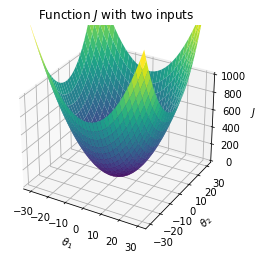
\includegraphics[width=70mm,scale=0.5]{images/gradient_descent_images/3dplot.png}
        
        \caption*{The "height"of your plot in 3D, is, again, your output! You want to move \textbf{downhill}.}
    \end{figure}
        
    \subsection{Multivariable Local Approximation (Review)}
    
        Again, we rely on \textbf{calculus}. We want to move up to having more parameters: more \textbf{dimensions}. 
        
        Before, in 1-D, we found that, if you \textbf{zoomed} in enough on a function (using a "\textbf{local} view"), we could \textbf{approximate} it as a \textbf{straight line}, and move up or down that slope.
        
        There are \textbf{two} ways we can \textbf{approximate} like we want to in 2-D:
            \note{Remember that, by 2-D, we mean two \textbf{parameters}/inputs to $J$. If we add in the \textbf{height} of our function, that means our plot will \textbf{look} like 3-D!}
        
        \begin{itemize}
            \item First, we could turn it back into 1-D: we remove one variables.
            
            We do this by turning one variable constant: take $\theta_2=0$. Now, we have one free variable $\theta_1$. Same as 1-D.\\
        \end{itemize}
        
        \begin{concept}
            We can \gren{reduce} the number of \purp{variables} we have to work with, by holding some of them \gren{constant}. That way, we have a \purp{simpler} problem to work with.
            
            This is \purp{the same} as taking a single 2-D plane in a 3-D plot.
        \end{concept}
        
        \begin{figure}[H]
                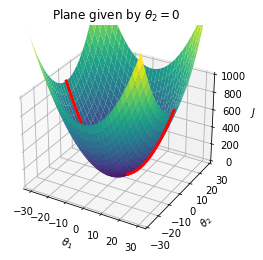
\includegraphics[width=70mm,scale=0.5]{images/gradient_descent_images/theta2_eq_0_unsliced.png}
                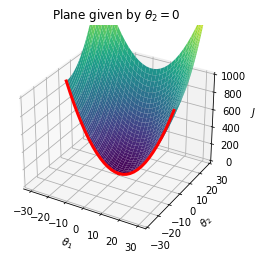
\includegraphics[width=70mm,scale=0.5]{images/gradient_descent_images/theta2_eq_0_sliced.png}
            
            \caption*{If we focus on a single plane of this surface, we end up with a \textbf{parabola}.}
        \end{figure}
        
        We can do the same the other way: we take $\theta_1=0$, and now we have a 1-D problem in $\theta_2$.
        
        \begin{figure}[H]
                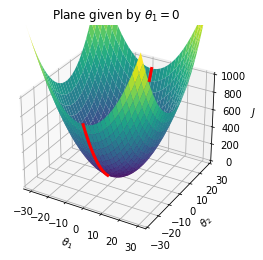
\includegraphics[width=70mm,scale=0.5]{images/gradient_descent_images/theta1_eq_0_unsliced.png}
                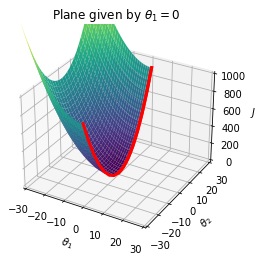
\includegraphics[width=70mm,scale=0.5]{images/gradient_descent_images/theta1_eq_0_sliced.png}
            
            \caption*{We can slice along the other axis as well!}
        \end{figure}

        Along each \textbf{axis}, $\theta_1$ and $\theta_2$, you can \textbf{approximate} our function as \textbf{two} different straight lines. Which leads into our next point...
        
        \begin{itemize}
            \item Second way: if we take the two perpendicular \textbf{lines} we got from each dimension, we can combine them into a \textbf{plane}.\\
        \end{itemize}
        
        \begin{concept}
            If we have \vocab{two input variables} (a 2-D problem), we can \purp{approximate} our surface as a \vocab{plane} if we \gren{zoom} in enough.
        \end{concept}
        
        These \textbf{approximations} will allow us to \textbf{optimize}.

    \subsection{2-D: One dimension at a time}
        
        How do we \textbf{improve} our function $J$? Now that we have \textbf{two} dimensions, we have to store our change $\Delta \theta$ in a \textbf{vector}:
        
        \begin{equation}
            \Delta \theta
            =
            \begin{bmatrix}
                  \Delta \theta_1 \\ \Delta \theta_2 
            \end{bmatrix}
        \end{equation}
        
        This \textbf{complicates} things: we have two different things to consider \textbf{at once}.
        
        Well, the \textbf{simplest} way would be to treat it as a \textbf{1-D} problem, and do exactly what we did \textbf{before}. 
            \note{Note that we switched to \textbf{partial} derivatives, because we have \textbf{multiple} input variables $\theta_i$.}
        
        \begin{equation}
            \Delta \theta_1 = \pderiv{J}{\theta_1}
        \end{equation}
        
        Writing this in our \textbf{new} notation, we get:
        
        \begin{equation}
            \Delta \theta
            =
            - \eta 
            \begin{bmatrix}
                  \pderivslash{J}{\theta_1} \\ 0 
            \end{bmatrix}
        \end{equation}
        
        And then we would take a \textbf{step}, moving along the $\theta_1$ \textbf{axis}.
        
        \begin{figure}[H]
            \centering
                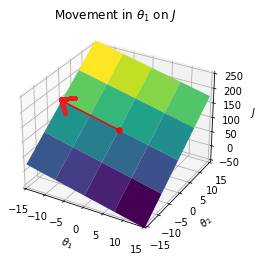
\includegraphics[width=70mm,scale=0.5]{images/gradient_descent_images/theta1_movement_plane.png}
            \caption*{We can move along $\theta_1$ just like on a line.}
        \end{figure}
        
        What if we treated this as a 1-D problem for the \textbf{other} variable, $\theta_2$?
        
        \begin{equation}
            \Delta \theta
            =
            - \eta 
            \begin{bmatrix}
                  0 \\ \pderivslash{J}{\theta_2} 
            \end{bmatrix}
        \end{equation}
        
        With this equation, we would be \textbf{moving} along the $\theta_2$ axis.
        
        \begin{figure}[H]
            \centering
                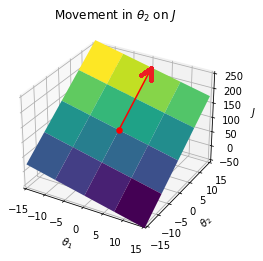
\includegraphics[width=70mm,scale=0.5]{images/gradient_descent_images/theta2_movement_plane.png}
            \caption*{We can do the same with $\theta_2$.}
        \end{figure}
        
        Why not move in \textbf{both} directions \textbf{at once}? We can \textbf{combine} our two derivatives: we'll add up our two steps.
        
        \textbf{Linearity} means that I can \textbf{add} them up without anything \textbf{weird} happening.
            \note{The relevant linearity rule: $L(x+y)=L(x)+L(y)$. In other words: taking two separate steps is the same as one big step.}
        
        \begin{equation}
            \Delta \theta
            =
            - \eta 
            \begin{bmatrix}
                  \pderivslash{J}{\theta_1} \\ 0 
            \end{bmatrix}
            - \eta 
            \begin{bmatrix}
                  0 \\ \pderivslash{J}{\theta_2} 
            \end{bmatrix}
        \end{equation}
        
        These can be combined because we're treating our function as a \textbf{flat} plane: if I move in the $\theta_1$ direction first, it doesn't change the $\theta_2$ slope, and vice versa.
        
        \begin{figure}[H]
        \centering
            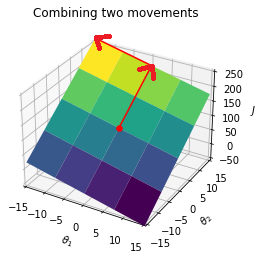
\includegraphics[width=70mm,scale=0.5]{images/gradient_descent_images/thetaboth_movement_plane.png}

            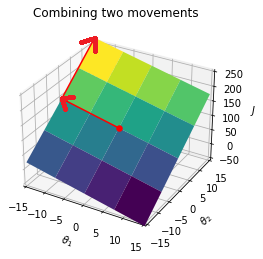
\includegraphics[width=70mm,scale=0.5]{images/gradient_descent_images/thetaboth_movement_plane_reversed.png}
                
            \caption*{Our plane being flat means we can take both operations, back-to-back! Notice that the order doesn't matter.}
        \end{figure}
        
        \begin{equation}
            \Delta \theta
            =
            - \eta 
            \begin{bmatrix}
                  \pderivslash{J}{\theta_1} \\ \pderivslash{J}{\theta_2} 
            \end{bmatrix}
        \end{equation}
        
        So, let's use that to optimize:\\
        
        \begin{kequation}
            In \vocab{2-D}, you can optimize your function $J$ using this rule:
            
            \begin{equation*}
                \red{ \theta_{new} } =  \blu{ \theta_{old} } 
                - \grn{ \eta } 
                \underbrace{
                    \begin{bmatrix}
                          \pderivslash{J}{ \blu{\theta_1} } \\ 
                          \pderivslash{J}{ \blu{\theta_2} } 
                    \end{bmatrix}
                }_{ \text{Using } \blu{ \theta_{old} } }
            \end{equation*}
            
            This is our \vocab{gradient descent} rule for 2-D.
        \end{kequation}
        
        This sort of approach makes some \textbf{sense}: if $\pderiv{J}{\theta_1}$ is \textbf{bigger} than $\pderiv{J}{\theta_2}$, that means that you can get \textbf{more benefit} from moving in the $\theta_1$ direction than $\theta_2$.
        
        So, in that case, your step will move more in the $\theta_1$ direction: it's a more \textbf{efficient} way to get a \textbf{better} hypothesis!
        
        But for now, we \textbf{don't know} that this is necessarily the \textbf{optimal} way to change $\theta$ - we'll explore that later.
        
        
    \subsection{Gradient Descent in n-D}
    
        This idea can be built up in \textbf{any number} of dimensions: each variable $\theta_k$ creates a \textbf{different} line we can use to \textbf{approximate}.
        
        And, we can combine them into a \textbf{flat} hyperplane: so, we can \textbf{add up} all of the different \textbf{derivatives}.\\
        
        \begin{kequation}
            In \vocab{n-D}, you can optimize your function $J$ using this rule:
            
            \begin{equation*}
                \red{ \theta_{new} } =  \blu{ \theta_{old} } 
                - \grn{ \eta } 
                \underbrace{
                    \begin{bmatrix}
                          \pderivslash{J}{ \blu{\theta_1} } \\ 
                          \pderivslash{J}{ \blu{\theta_2} } \\
                          \vdots \\
                          \pderivslash{J}{ \blu{\theta_d} } \\
                    \end{bmatrix}
                }_{ \text{Using } \blu{ \theta_{old} } }
            \end{equation*}
            
            This is our \vocab{generalized gradient descent} rule.
        \end{kequation}

    \subsection{The Gradient}
    
        We call this \textbf{gradient} descent because that right term \textbf{is} the gradient!\\
        
        \begin{definition}
            
            The gradient can be written as
            
            \begin{equation*}
                \nabla_\theta J 
                = 
                \begin{bmatrix}
                      \pderivslash{J}{ \blu{\theta_1} } \\ 
                      \pderivslash{J}{ \blu{\theta_2} } \\
                      \vdots \\
                      \pderivslash{J}{ \blu{\theta_d} } \\
                \end{bmatrix}
                =
                \deriv{J}{\theta}
            \end{equation*} 
        \end{definition}
        
        So, our rule can be rewritten (for the last time) as:\\
        
        \begin{kequation}
            The \vocab{gradient descent} rule can be generally written as:
            
            \begin{equation*}
                \red{ \theta_{new} } =  \blu{ \theta_{old} } 
                - \grn{ \eta } 
                \nabla_\theta J ( \blu{ \theta_{old} } )
            \end{equation*}
            
            $\blu{ \theta_{old} }$ is the input to $\nabla_\theta J$, not multiplication!
            
            \begin{equation*}
                \red{ \theta_{new} } =  \blu{ \theta_{old} } 
                - \grn{ \eta } 
                J'( \blu{ \theta_{old} } )
            \end{equation*}
        \end{kequation}
        
        Now, is $\nabla_\theta J$ the \textbf{optimal} way to improve(optimize) $\theta$? Let's find out.
    
    \subsection{The Plane Approximation}
        
        So, what \textbf{is} the best direction? Which way will increase/decrease $J$ \textbf{fastest?} 
        
        \textit{Is} it the gradient? Let's explore a bit to figure that out. Let's look at our plane, and see what hints it might provide:
            \note{For explanation purposes, we'll assume 2-D, but the explanation extends to n-D.}\\
        
        \begin{concept}
            Assume your function is, at least locally, a \vocab{flat plane}.

            \begin{itemize}
                \item A \purp{flat plane} has only \gren{one} direction of \vocab{maximum increase}: this is the direction you might call, "directly \gren{uphill}" if you think of elevation.
                
                \item The \gren{opposite} direction is the direction of \purp{maximum decrease}, or "\gren{downhill}".
                
                \item If you move at a \vocab{right angle} to the "best" direction (maximum increase/decrease), the function \purp{will not change}. In elevation, you stay at the \gren{same height}!
            \end{itemize}
        \end{concept}
        
        This is useful! We can \textbf{break down} any direction into the part that \textbf{affects} our function $J$, and the part that \textbf{doesn't}.
            \note{In the n-D case, we have \textbf{more} perpendicular directions. But, all of them have \textbf{no effect}!}
        
        
    
    \subsection{The Optimal Direction: The Gradient}
    
        How do we get the optimal direction?
        
        The \textbf{total} change in $J$ is gotten by just \textbf{adding} the change in each direction (thank you planes!):
        
        \begin{figure}[H]
        
                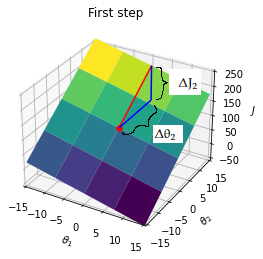
\includegraphics[width=70mm,scale=0.5]{images/gradient_descent_images/first_step.png}
                
                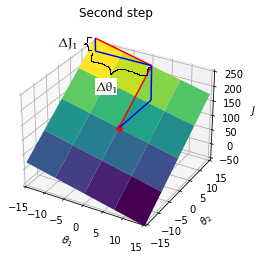
\includegraphics[width=70mm,scale=0.5]{images/gradient_descent_images/second_step.png}
                
            \caption*{You can add up the results of our two steps: $\Delta J_2$ and $\Delta J_1$.}
        \end{figure}
        
        \begin{equation}
            \Delta J \approx \Delta J_1 + \Delta J_2
        \end{equation}
        
        Let's convert that using derivatives:
        
        \begin{equation}
            \Delta J \approx
            \Delta \theta_1 \pderiv{J}{\theta_1} +
            \Delta \theta_2 \pderiv{J}{\theta_2}
        \end{equation}
        
        Now we've got a useful equation: the total change. As a bonus we can see a clear \textbf{pattern} ($\nth{i}$ $\theta$ matches $\nth{i}$ derivative). 
        
        So, \textbf{condense} this pattern, like we did for our linear model: using a \textbf{dot product}.
        
        \begin{equation}
            \Delta J 
            \approx 
            \begin{bmatrix}
              \Delta \theta_1 \\ \Delta \theta_2
            \end{bmatrix}
            \cdot
            \begin{bmatrix}
                \pderivslash{J}{ \theta_1}  \\ 
                \pderivslash{J}{ \theta_2 } 
            \end{bmatrix}
            =
            \Delta \theta \cdot \nabla_\theta J
        \end{equation}
        
        The \textbf{gradient} shows up! Interesting. But what does that \textbf{mean}?
        
        Well, we want to \textbf{maximize} (or minimize!) our $\Delta J$. How do we maximize a \textbf{dot product}?
        
        By making sure the directions are \textbf{the same}! So, we can confirm that the \textbf{gradient} gives us the \textbf{best} direction.
        
        So, all we have to do is to \textbf{flip} the sign to \textbf{minimize} $\Delta J$.
            \note{And so, gradient descent is already complete!}\\
        
        \begin{concept}
            The \vocab{gradient} $\nabla J$ is the \vocab{direction of greatest increase} for $J$.
            
            That means means the opposite direction $-\nabla J$ is the \vocab{direction of greatest decrease} in $J$.
        \end{concept}
        
        This is the single \textbf{most important concept} in this entire chapter!
        
        
    \subsection{Termination Condition}
    
        We can still use our termination conditions from before, but we need to be careful to make sure they extrapolate to n-D.
        
        \begin{itemize}
            \item Stop after a fixed T steps.
                \begin{itemize}
                    \item Nothing to change here. 
                        \note{We don't use this one often, though!}
                \end{itemize}
                
            \item Stop when $\norm{\theta}$ isn't changing much: $\norm{\Delta \theta} < \epsilon$, for example.
                \begin{itemize}
                    \item We just had to replace \textbf{absolute} value with \textbf{magnitude}.
                \end{itemize}
                
            \item Stop when the derivative is small: $\abs{J'(\theta)} < \epsilon$
            
                \begin{itemize}
                    \item Nothing to change here.
                \end{itemize}
        \end{itemize}

    \subsection{Another explanation of gradient (OPTIONAL)}
    
        Some students may not like the \textbf{first} explanation given for why gradient is the \textbf{direction of greatest increase}. So here, we use a slightly \textbf{different} approach, one that's more \textbf{geometric}. 
        
        Feel free to skip this section if you are not interested.
        
        We look at a random vector, $\Delta \theta$ - no assurances about how good or bad it is.
        
        Currently, our vector \textbf{components} are based on $\theta_1$ and $\theta_2$. But, we want to \textbf{switch} perspectives.
        
        Our vector can \textbf{also} be broken up into \textbf{parts} based on whether it \textbf{affects} $J$. This will let us take a \textbf{look} at the "best direction" we're trying to \textbf{find}.
        
        \begin{itemize}
            \item Uphill: the "best" direction $\hat{u}_{best}$ (magnitude $\Delta B$)
            
            \item Same height: the direction with no effect, $\hat{u}_{none}$ (magnitude $\Delta N$)
        \end{itemize}
        
        \begin{equation}
            \Delta \theta
            =
            \underbrace{
                \Delta B \red{ \hat{u}_{best} }
            }_{\text{Full effect on J}} 
            + 
            \underbrace{
                \Delta N \red{ \hat{u}_{none} }
            }_{ \text{No effect on J} } 
        \end{equation}
        
        So, all of the change in $J$ just comes from $\hat{u}_{best}$. We \textbf{don't care} about the other direction!\\
        
        \begin{concept}
            In a \vocab{local planar approximation}, the \purp{only} component of $\Delta \theta$ that \gren{affects} $J$ is the \vocab{direction of greatest increase}, $\hat{u}_{best}$.
            
            So, we can determine $\Delta J$ using \purp{only that component}.
        \end{concept}
        
        But, $\nabla_{\theta} J$ \textbf{also} gives us change in $\Delta J$: it contains all of the \textbf{derivatives}, and thus gives us the effect $\theta$ has on $\Delta J$.
        
        So we can find:
        
        \begin{equation}
            \Delta \theta \cdot \deriv{J}{\theta} 
            = \Delta J = 
            \left( 
                \Delta \theta \cdot \hat{u}_{best} 
            \right) 
            \deriv{J}{B}
        \end{equation}
        
        $\Delta \theta$ is being dotted with both the \textbf{gradient} and the \textbf{best direction}: they both give the change in $J$. To keep the \textbf{dot product} consistent as $\Delta \theta$ changes, they need to be in the \textbf{same direction}.

\pagebreak
%%%%%%%%%%%%%%%%%%%%%%%%%%%%%%%%%%%%%%%%%%%%%%%%%%%%%%%%%%%%%%%%%%%%%%%%%%%%%%%%%%%%%%%%%%%
\section{Application to Regression}
    
    One nice thing about \textbf{gradient descent} is that it is \textbf{easy} to switch the kind of problem you're applying it to: all you need is your \textbf{parameters}(s) $\theta$, and a function to optimize, $J$.
    
    From there, you can just \textbf{compute} the gradient.

    \subsection{Ordinary Least Squares}
        
        Our \textbf{loss} function is
        
        \begin{equation}
            J(\theta,\theta_0) = 
            \frac{1}{n}  \sum_{i=1}^n 
            \left( \red{ (\theta^T} \blu{\ex{x}{i}} \red{ + \theta_0) } 
            - \blu{\ex{y}{i}} \right)^2 
        \end{equation}
            
        Or, in \textbf{matrix} terms,
            \note{Including the appended row of 1's from before.}
        
        \begin{equation*}
            J = \frac{1}{n}
                \left( \red{ \Xt \theta  - \Yt } \right)^T
                \left( \red{ \Xt \theta  - \Yt } \right) 
        \end{equation*}
        
        Our gradient, according to \textbf{matrix derivative} rules, is
        
        \begin{equation}
            \nabla_\theta J(\theta) = 
                \frac{2}{n} \Xt^T
                \left( \red{ \Xt \theta  - \Yt } \right) 
        \end{equation}
        
        Before, we set it equal to \textbf{zero}. But here, we can instead take \textbf{steps} towards the solution, using \textbf{gradient descent}.
        
        We could use the \textbf{matrix} form, but sometimes it's easier to use a \textbf{sum}. Fortunately, derivatives are easy with a sum. If so, here's \textbf{another} way to write it:
        
        \begin{equation}
            \nabla_\theta J(\theta) 
            = 
            \frac{2}{n} \sum_{i=1}^n
            \left(
                \red{\theta^T} \blu{\ex{x}{i}} - \blu{\ex{y}{i}}
            \right)
            \blu{\ex{x}{i}}
        \end{equation}
        
        Either way, we use gradient descent \textbf{normally}:
            \note{Remember that $\blu{ \theta_{old} }$ is an \textbf{input} to the gradient, not multiplied by it!}
        
        \begin{equation*}
            \red{ \theta_{new} } 
            =  
            \blu{ \theta_{old} } 
            - \grn{ \eta } 
            \nabla_\theta J ( \blu{ \theta_{old} } )
        \end{equation*}
        
        Using $\ex{\theta}{t}$ notation:
        
        \begin{equation*}
            \red{ \ex{\theta}{t} } = 
            \blu{ \ex{\theta}{t-1} } -
            \grn{\eta} \nabla_\theta J ( \blu{ \ex{\theta}{t-1} })
        \end{equation*}
        
    \subsection{Ridge Regression}
    
        Ridge regression is similar. 
        
        \begin{equation*}
                J(\theta) 
                = 
                \frac{1}{n}  \sum_{i=1}^n 
                \left( 
                    \underbrace{
                        \red{(\theta^T \ex{x}{i}  
                        + \theta_0)}
                    }_{guess}
                    - \underbrace{
                        \blu{\ex{y}{i}} 
                    }_{answer}
                \right)^2 
                + 
                \underbrace{
                    \pur{ \lambda \norm{\theta}^2 }
                }_{Regularizer}
            \end{equation*}
        
        However, we have to treat $\theta_0$ as \textbf{separate} from our other data points, because of \textbf{regularization}: remember that it \textbf{doesn't} apply to $\theta_0$.
        
        For $\theta$:
        
        \begin{equation}
            \nabla_\theta J_\text{ridge}(\theta, \theta_0)
            =
            \frac{2}{n}\sum_{i=1}^n
            \left(
                \red{(\theta^T} \blu{\ex{x}{i}} + \red{\theta_0)}
                - 
                \blu{\ex{y}{i}}
            \right)
            \blu{\ex{x}{i}}
            +
            \pur{2 \lambda \theta}
        \end{equation}
        
        For $\theta_0$:
        
        \begin{equation}
            \pderiv{J_\text{ridge}(\theta, \theta_0)}{\theta_0} 
            =
            \frac{2}{n}\sum_{i=1}^n
            \left(
                \red{(\theta^T} \blu{\ex{x}{i}} + \red{\theta_0)}
                - 
                \blu{\ex{y}{i}}
            \right)
        \end{equation}
        
        Notice that we used a \textbf{gradient} for our vector $\theta$, but since $\theta_0$ is a single variable, we just used a \textbf{simple derivative}!\\
        
        \begin{concept}
            The \vocab{gradient} $\deriv{J}{\theta}$ must have the \vocab{same shape as $\theta$}: this shape-matching is why we can easily \gren{subtract} it during gradient descent.
            
            \begin{equation*}
                \underbrace{
                    \red{ \theta_{new} } 
                }_{(d \times 1)}
                =  
                \underbrace{
                    \blu{ \theta_{old} } 
                }_{(d \times 1)}
                - \grn{ \eta } 
                \underbrace{
                    \nabla_\theta J ( \blu{ \theta_{old} } )
                }_{(d \times 1)}
            \end{equation*}
        \end{concept}
    
    \subsection{Computational Gradient}
    
        Sometimes, we \textbf{can't} easily find the \textbf{equation} for our gradient: maybe our loss isn't a simple \textbf{equation}, or we have some \textbf{other} kind of problem. So, rather than getting the \textbf{exact} gradient, we \textbf{approximate} it.
        
        But how do we \textbf{approximate} the gradient? Well, first, we could \textbf{reference} how we approximate a \textbf{simple derivative}.
            \note{A derivative is just a 1-D gradient, after all!}
            
        The definition of the \textbf{derivative} can be gotten as 
        
        \begin{equation}
            f'(x) = \lim_{h \rightarrow 0} \frac{f(x+h)-f(x)}{h}
        \end{equation}
        
        But, what if we can't take the \textbf{limit}? Or, we just don't \textbf{want} to? 
        
        We can \textbf{approximate} by taking $h$ to be a small, \textbf{finite} number.
        
        Instead of $h$, we'll call this $\delta$.
        
        \begin{concept}
            When \vocab{approximating} the derivative, we can choose a \purp{small} finite width to measure, called $\delta$, so that
            
            \begin{equation}
                \deriv{f}{x} \approx
                \frac{f(x+\delta)-f(x)}{\delta} , \qquad \delta << 1
            \end{equation}
        \end{concept}
        
        So, let's \textbf{extend} that to the \textbf{gradient}:
        
        \begin{equation}
            \nabla_\theta J 
            = 
            \begin{bmatrix}
                  \pderivslash{J}{ \blu{\theta_1} } \\ 
                  \pderivslash{J}{ \blu{\theta_2} } \\
                  \vdots \\
                  \pderivslash{J}{ \blu{\theta_d} } \\
            \end{bmatrix}
        \end{equation}
        
        Luckily, the \textbf{gradient} is just a bunch of derivatives \textbf{stacked} in a \textbf{vector}! 
        
        So, we can just \textbf{compute} each of them \textbf{separately}, and then put them together.
        
        Let's show how we'd \textbf{write} that in \textbf{vector} form, for just one of them. We want something like
        
        \begin{equation}
            \underbrace{
                J'(\theta) \approx
                \frac{J(\theta+\delta)-f(\theta)}{\delta} 
            }_{\text{Not correct, but closer}}
        \end{equation}
        
        This isn't quite right, because a \textbf{scalar} $\delta$ would \textbf{add} to \textbf{every term}.
        
        We \textbf{only} want to shift \textbf{one} variable at a time, so we can do a \textbf{simple} derivative.
        
        Let's say we want $\derivslash{J}{\theta_1}$. We would \textbf{only} want to add $\delta$ to $\theta_1$: the other parameters are \textbf{unchanged}.
        
        So, we \textbf{can't} add a \textbf{scalar}. Instead, we need a $(d \times 1)$ vector: one term to \textbf{separately} add to each $\theta_k$ term.
        
        \begin{equation}
            \Delta \theta 
            = 
            \begin{bmatrix}
                \Delta \theta_1 \\ \Delta \theta_2 \\ \vdots \\ \Delta \theta_d
            \end{bmatrix}
        \end{equation}
        
        We want most terms \textbf{unchanged}, so we'll \textbf{add 0} to each of them, and we'll add $\delta$ to the one term we want to \textbf{edit}.
        
        \begin{equation}
            \Delta \theta 
            = 
            \begin{bmatrix}
                \delta \\ 0 \\ \vdots\\ 0 \\ 0
            \end{bmatrix}
        \end{equation}
        
        We'll \textbf{create} one of these vectors for each \textbf{dimension}. We'll give them a special \textbf{name}: $\delta_k$, for the $\nth{k}$ dimension.
        
        \begin{equation}
            \delta_1 
            = 
            \begin{bmatrix}
                \delta \\ 0 \\ \vdots\\ 0 \\ 0
            \end{bmatrix}
            \qquad
            \delta_2 
            = 
            \begin{bmatrix}
                0 \\ \delta \\ \vdots\\ 0 \\ 0
            \end{bmatrix}
            \qquad
            \delta_{d-1} 
            = 
            \begin{bmatrix}
                0 \\ 0 \\ \vdots\\ \delta \\ 0
            \end{bmatrix}
            \qquad
            \delta_{d} 
            = 
            \begin{bmatrix}
                0 \\ 0 \\ \vdots\\ 0 \\ \delta
            \end{bmatrix}
        \end{equation}
        
        Finally, we'll \textbf{divide} by $\delta$. We have what we need for our full equation:\\
        
        \begin{kequation}
            In order to \vocab{computationally find the gradient}, you need to find the \purp{partial derivative} for each term $\theta_k$.
            
            \begin{equation*}
                \deriv{J}{\theta_k} \approx
                \frac{J(\theta+\delta_k)-f(\theta)}{\delta}
            \end{equation*}
            
            Where 
            
            \begin{itemize}
                \item $\delta$ is a small positive number
                \item $\delta_k$ is the $(d \times 1)$ \gren{column vector} with a $\delta$ in the $\nth{k}$ row, and a 0 in every other row.
            \end{itemize} 
        \end{kequation}

    
    \subsection{Problems with Gradient Descent}
        
        Gradient descent is very handy, but it's important to be aware of some of its \textbf{problems}.
        
        We've discussed a couple: diverging, oscillating, and converging slowly. We also have to worry about \textbf{local minima} that aren't as good as other answers.
        
        But there's also a \textbf{limitation}: our loss function has to be \textbf{smooth} and \textbf{differentiable}. If it isn't, we can't take the \textbf{gradient} of it.\\
        
        \begin{concept}
            \vocab{Gradient descent} requires for your \gren{functions} to be (at least mostly) \vocab{smooth and differentiable.}
        \end{concept}
        
        Our \textbf{answer} is also only as good as our \textbf{loss function}: if our loss function is not good for what we actually want to \textbf{accomplish}, then we can easily create a \textbf{bad} model.
        
\pagebreak
%%%%%%%%%%%%%%%%%%%%%%%%%%%%%%%%%%%%%%%%%%%%%%%%%%%%%%%%%%%%%%%%%%%%%%%%%%%%%%%%%%%%%%%%%%%
\section{Stochastic Gradient Descent}

    \subsection{Another problem with gradient descent}
        One \textbf{advantage} we mentioned for gradient descent at the beginning of the chapter is that we can \textbf{stop early} if we think we're done, saving on \textbf{time}.
        
        This is helpful for really \textbf{large} datasets, and it's also more \textbf{computationally manageable} than inverting a gigantic $XX^T$ matrix.
        
        But, we \textbf{haven't} taken \textbf{full advantage} of it: above, we used a \textbf{sum} to get our gradient - we're assuming we'll use all of our \textbf{data points}.
        
        But, what if we don't want to have to use all of them at once? That might be \textbf{expensive}. 
        
        And in fact, there are \textbf{other} reasons not to: maybe the gradient will change directions after only a \textbf{small} distance. 
        
        Right now, we're getting \textbf{lots of data} before even taking a \textbf{single step}: if we start moving \textbf{immediately}, our program could \textbf{adapt} to the "terrain" more quickly!
        
    \subsection{A better way: stochastic GD}
        
        Instead, why wait until we have \textbf{added} up over all the data? We could just \textbf{compute} the gradient over \textbf{one} data point \textbf{at a time}. In fact, to be fair, we'll do it \textbf{randomly}. 
            \note{To compensate, our steps will have to be \textbf{smaller}!}
        
        But wait, this \textbf{seems} like it would be \textbf{less} effective - after all, how much does \textbf{one} data point tell you? 
        
        Well, even if it isn't much, this isn't very \textbf{different} from adding them up all at \textbf{once}: in \textbf{theory}, taking lots of \textbf{little} steps should average out to the \textbf{same} information as if we do it all at once.\\
        
        \begin{definition}
            \vocab{Stochastic Gradient Descent (SGD)} is the process of applying \purp{gradient descent} on \gren{randomly} selected data points.
            
            This should \gren{average} out to being \gren{similar} to regular (batch) gradient descent, but the \purp{randomness} often lets it improve \purp{faster} and \gren{avoid} some common problems.
        \end{definition}
            
        \note{Stochastic is just a very mathematically precise word for "random".}
        
        There are more possible benefits, too: \textbf{randomly} choosing data points adds some \textbf{noise}, and random movement might be able to pull us out of local minima we don't want.
            \note{We mean "noise" in the signals sense: random \textbf{variation} in our data that \textbf{isn't} part of what we're trying to pay attention to: in this case, the \textbf{distribution}.}
            
        This sort of \textbf{noise} and \textbf{randomness} can make it hard for our model to \textbf{perfectly} fit the training data: this can reduce \textbf{overfitting}, too!
            \note{For example, it's hard to focus on the details of someone's eyelashes (unimportant details) if your vision is blurry.}
            
        \begin{concept}
            There are many \vocab{benefits} to \vocab{SGD} (Stochastic Gradient Descent) over regular BGD (Batch Gradient Descent).
            
            \begin{itemize}
                \item SGD can sometimes \gren{learn} a good model \purp{without} using all of our \gren{data}, which can \vocab{save us time} when data sets are \purp{too large}.
                    \begin{itemize}
                        \item It can also let us address problems \gren{early} if the model \purp{isn't} improving.
                    \end{itemize}
                    
                \item The noise produced by the random sampling in SGD can sometimes help it \vocab{avoid local minima} that aren't very good models, 
                    \begin{itemize}
                        \item This is because the model might be moved in a \purp{random direction} in \gren{parameter space}, and randomly \gren{pulled out} of that minimum, even if BGD would have gotten \purp{stuck}.
                    \end{itemize}
                    
                \item The noise also \vocab{reduces overfitting}, because it's \gren{harder} for the model to \purp{memorize} the exact details of the \purp{distribution}.
            \end{itemize}
        \end{concept}
        
    \subsection{Ensuring Convergence}
    
        How do we make sure that our SGD method converges? We need some kind of termination criteria. Thankfully, there's a useful theorem on the matter:\\
        
        \begin{theorem}
            SGD \purp{converges} with \textit{probability one} to the \purp{optimal} $\Theta$ if
            
            \begin{itemize}
                \item $f$ is convex
            \end{itemize}
            
            And our step size(learning rule) $\eta(t)$ follows these rules:
            
            \begin{equation*}
                \sum_{t=1}^{\infty} \eta(t) = \infty
                \qquad \qquad
                and
                \qquad \qquad
                \sum_{t=1}^{\infty} \eta(t)^2 < \infty
            \end{equation*}
        \end{theorem}
        
        Why these rules? Let's see:
        
        \begin{itemize}
            \item The \textbf{first} rule is for the \textbf{same} reason as for regular BGD: if it isn't \textbf{convex}, we can get stuck in \textbf{local minima}, or if it's \textbf{concave}, decrease \textbf{forever}.
            
            \item The \textbf{second} rule means that your steps need to add up to an \textbf{infinite distance}: this allows you to reach \textbf{any} possible point in your \textbf{parameter space}.
            
            \item The \textbf{third} one is a bit \textbf{trickier}, but basically means the steps need to get \textbf{smaller}, so we can approach the \textbf{minimum} (otherwise we might \textbf{diverge}!)
        \end{itemize}
        
        One option is $\eta(t)=1/t$. But often, we use rules that \textbf{decrease} more \textbf{slowly}, so that it doesn't take as \textbf{long}.
            \note{But technically, we're no longer guaranteed convergence!}

\section{Terms}
    
    \begin{itemize}
        \item Gradient Descent
        \item Parameter Space
        \item Local view (Calculus)
        \item Linear Function Approximation
        \item Planar Function Approximations
        \item Convergence
        \item Divergence
        \item Oscillation
        \item Step size
        \item Termination Condition
        \item Concavity/Convexity
        \item Global Minimum
        \item Local Minimum
        \item Initialization
        \item Gradient (Direction of Maximum Increase)
        \item Gradient Descent Rule
        \item Gradient Shape
        \item Gradient Approximation
        \item Stochastic Gradient Descent
        \item Batch Gradient Descent
        \item BGD Convergence Theorem
        \item SGD Convergence Theorem
    \end{itemize}